% ============================================================================
% FILE: sections/02_design.tex
% PURPOSE: การออกแบบทั้ง 3 ด้าน Mechanical / Electronics / Control
% ============================================================================

\section{การออกแบบระบบ (System Design)}
\label{sec:system_design}

% ============================================================
\subsection{การออกแบบเชิงกล (Mechanical Design)}
\label{subsec:mechanical_design}
% ============================================================

\subsubsection{สถาปัตยกรรมเชิงกลโดยรวม}
\begin{figure}[H]
    \centering
    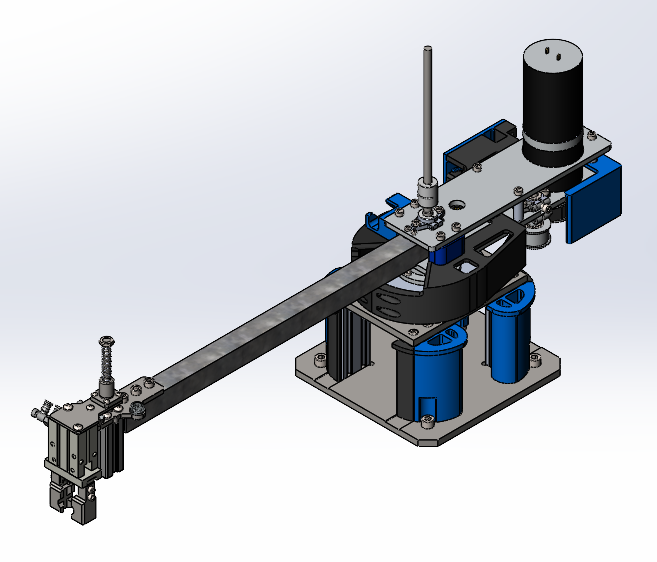
\includegraphics[width=0.8\textwidth]{images/Full_CAD.png}
    \caption{CAD Assembly ของระบบเชิงกล}
    \label{fig:cad_assembly_overall}
\end{figure}

% ------------------------------------------------------------
\subsection{การคำนวณเพลา (Shaft Calculation)}
\label{subsec:shaft_calc}
% ------------------------------------------------------------

การคำนวณขนาดเพลาดำเนินการตามทฤษฎี
Maximum Shear Stress (ASME Code)
เพื่อพิสูจน์ว่าเพลาหลักของ Azimuth Joint
สามารถรับแรงบิดและโมเมนต์ดัดรวมได้อย่างปลอดภัย

\subsubsection{สถาปัตยกรรมระบบและกลไกรับแรง}

ระบบเพลาประกอบด้วย 3 ชิ้นส่วนหลัก ได้แก่
เพลาขับหลัก (Main Shaft) ทำหน้าที่รับแรงดัด
และแรงบิดจากโหลด,
ตลับลูกปืนตัวบน (Taper Roller Bearing)
รับแรงในแนวรัศมีและแนวแกนเป็นหลัก
และถือเป็นจุดวิกฤตความเค้น และ
ตลับลูกปืนตัวล่าง (Deep Groove Ball Bearing)
ทำหน้าที่ประคองเพลา (Secondary Support)

% [รูป Free Body Diagram ของระบบเพลา]
% \begin{figure}[H]
%   \centering
%   \includegraphics[width=0.75\textwidth]{images/shaft_fbd.png}
%   \caption{Free Body Diagram ของระบบเพลา
%            แสดงแรงและโมเมนต์ที่กระทำที่จุดวิกฤต}
%   \label{fig:shaft_fbd}
% \end{figure}

\subsubsection{พารามิเตอร์และคุณสมบัติวัสดุ}

\begin{table}[H]
  \centering
  \caption{พารามิเตอร์ภาระโหลดของระบบเพลา}
  \label{tab:shaft_loads}
  \begin{tabular}{llll}
    \toprule
    พารามิเตอร์ & สัญลักษณ์ & ค่า & หน่วย \\
    \midrule
    มวลโหลดที่ปลายเพลา        & $m$        & 3.72   & kg \\
    น้ำหนักโหลดในแนวดิ่ง       & $W$        & 37.20  & N \\
    ระยะเยื้องศูนย์ด้านหน้า     & $L_{cg}$   & 46.63  & mm \\
    ความเร็วรอบ                 & $N$        & 85.00  & RPM \\
    แรงเหวี่ยงหนีศูนย์กลาง     & $F_c$      & 13.75  & N \\
    แรงดึงสายพานรวม            & $F_{belt}$ & 130.00 & N \\
    \midrule
    ระยะจาก Load ถึง ลูกปืนบน  & $L_1$      & 25.25  & mm \\
    ระยะจาก ลูกปืนบน ถึง ล่าง & $L_2$      & 37.25  & mm \\
    \bottomrule
  \end{tabular}
\end{table}

วัสดุที่เลือกใช้คือ Stainless Steel AISI 304
\begin{itemize}
  \item Yield Strength: $S_{yt} = 215$\,MPa
  \item Allowable Shear Stress:
        $\tau_d = 0.30 \times S_{yt}
               = 0.30 \times 215
               = 64.5$\,MPa
        (ตามมาตรฐาน ASME)
\end{itemize}

\subsubsection{การวิเคราะห์โมเมนต์ดัด}

\paragraph{โมเมนต์จากโหลดปลายเพลา (Overhang Bending Moment)}

โหลด 3.72\,kg ที่เยื้องศูนย์ 46.63\,mm
สร้างโมเมนต์ดัดคงที่ตลอดเวลาที่จุดลูกปืนบน

\begin{equation}
  M_{overhang} = (W + F_c) \times L_1
               = (37.20 + 13.75) \times 0.02525
               = 1.287\,\text{N}\cdot\text{m}
  \label{eq:shaft_m_overhang}
\end{equation}

\paragraph{โมเมนต์จากแรงดึงสายพาน (Belt Tension Moment)}

แรงสายพานกระทำที่ Pulley ผ่านแขนของโมเมนต์ $L_1$

\begin{equation}
  M_{belt} = F_{belt} \times L_1
           = 130.00 \times 0.02525
           = 3.283\,\text{N}\cdot\text{m}
  \label{eq:shaft_m_belt}
\end{equation}

\paragraph{โมเมนต์ดัดรวมสุทธิ (Worst-case Superposition)}

พิจารณา Worst-case โดยให้โมเมนต์ทั้งสองเสริมกัน

\begin{equation}
  M_{total} = M_{overhang} + M_{belt}
            = 1.287 + 3.283
            \approx 4.57\,\text{N}\cdot\text{m}
  \label{eq:shaft_m_total}
\end{equation}

% [รูป Bending Moment Diagram]
% \begin{figure}[H]
%   \centering
%   \includegraphics[width=0.75\textwidth]{images/shaft_bmd.png}
%   \caption{Bending Moment Diagram ของเพลา
%            แสดงโมเมนต์ดัดสูงสุดที่จุดวิกฤต}
%   \label{fig:shaft_bmd}
% \end{figure}

หมายเหตุ: รายงานการคำนวณระบุค่า
$M = 5.014$\,N$\cdot$m ซึ่งรวมผลของ
แรงเหวี่ยงและ Geometric factor
ที่คำนวณแบบ Vector Superposition
ครบถ้วนกว่าการประมาณข้างต้น
จึงใช้ $M = 5.014$\,N$\cdot$m
เป็นค่าสำหรับการออกแบบ

\subsubsection{แรงบิดของระบบ}

แรงบิดที่เกิดขึ้นในแกนเพลาจากการส่งกำลัง

\begin{equation}
  T = T_{arm} = 5.398\,\text{N}\cdot\text{m}
  \label{eq:shaft_torque}
\end{equation}

\subsubsection{การคำนวณขนาดเพลา (Shaft Sizing)}

\paragraph{Fatigue Design Factors}

เลือกค่าสัมประสิทธิ์ความปลอดภัยสำหรับ
สภาวะการทำงานแบบกระตุกเบา (Light Shock)
\begin{itemize}
  \item $C_m = 2.0$ (Bending Fatigue Design Factor)
  \item $C_t = 1.5$ (Torsional Fatigue Design Factor)
\end{itemize}

\paragraph{สมการ Maximum Shear Stress Theory}

สำหรับเพลาตัน (Solid Circular Shaft)
ตามมาตรฐาน ASME

\begin{equation}
  d_{min} = \left[
    \frac{16}{\pi \tau_d}
    \sqrt{(C_m M)^2 + (C_t T)^2}
  \right]^{1/3}
  \label{eq:shaft_diameter}
\end{equation}

แทนค่า

\begin{equation}
  d_{min} = \left[
    \frac{16}{\pi \times 64.5 \times 10^6}
    \sqrt{(2.0 \times 5.014)^2 + (1.5 \times 5.398)^2}
  \right]^{1/3}
\end{equation}

\begin{equation}
  d_{min} = \left[
    \frac{16}{\pi \times 64.5 \times 10^6}
    \sqrt{100.56 + 65.56}
  \right]^{1/3}
  = \left[
    \frac{16 \times 12.887}{2.027 \times 10^8}
  \right]^{1/3}
  = 10.59\,\text{mm}
  \label{eq:shaft_result}
\end{equation}

\subsubsection{การออกแบบ Step Shaft}

จากผลการคำนวณ $d_{min} = 10.59$\,mm
ออกแบบเป็น Step Shaft เพื่อรองรับการประกอบ
ชิ้นส่วนทางกล ดังตารางที่~\ref{tab:shaft_steps}

\begin{table}[H]
  \centering
  \caption{การประเมินความปลอดภัยของ Step Shaft
           แต่ละช่วง}
  \label{tab:shaft_steps}
  \begin{tabular}{lccl}
    \toprule
    ช่วงเพลา & ขนาด (mm) & $> d_{min}$ & หมายเหตุ \\
    \midrule
    ช่วงวิกฤต (ลูกปืนบน)
      & 17 & \checkmark & รับ Moment + Torque สูงสุด \\
    ช่วง Shoulder ลูกปืนล่าง
      & 14 & \checkmark & Shoulder รองรับ Bearing \\
    ช่วงกลาง
      & 12 & \checkmark & รับภาระลดลง \\
    ช่วงปลาย (เกลียว/Encoder)
      & 10 & ต่ำกว่าเล็กน้อย
      & ตำแหน่งนี้ไม่ใช่จุดวิกฤต \\
    ช่วงปลายสุด
      &  8 & ต่ำกว่าเล็กน้อย
      & ตำแหน่งนี้ไม่ใช่จุดวิกฤต \\
    \bottomrule
  \end{tabular}
\end{table}

% [รูป Step Shaft Drawing]
% \begin{figure}[H]
%   \centering
%   \includegraphics[width=0.85\textwidth]{images/shaft_drawing.png}
%   \caption{แบบ Step Shaft แสดงขนาดเพลา
%            แต่ละช่วงและตำแหน่งลูกปืน}
%   \label{fig:shaft_drawing}
% \end{figure}

การออกแบบ Step Shaft สอดคล้องกับผลการคำนวณ
โดยทุกช่วงที่รับภาระสูง ($\geq$12\,mm)
มีขนาดใหญ่กว่า $d_{min} = 10.59$\,mm
ส่วนช่วงปลายเพลา (8 และ 10\,mm)
แม้จะเล็กกว่าค่าคำนวณ แต่ตำแหน่งเหล่านี้
ไม่ได้อยู่ที่จุดวิกฤต จึงมีความปลอดภัยเพียงพอ

\begin{table}[H]
  \centering
  \caption{สรุปผลการคำนวณเพลา}
  \label{tab:shaft_summary}
  \begin{tabular}{lccl}
    \toprule
    พารามิเตอร์ & ค่า & หน่วย & หมายเหตุ \\
    \midrule
    Bending Moment $M$      & 5.014  & N$\cdot$m & Worst-case \\
    Torsional Moment $T$    & 5.398  & N$\cdot$m & จากระบบส่งกำลัง \\
    $d_{min}$ (คำนวณ)       & 10.59  & mm        & จุดวิกฤต \\
    $d_{actual}$ (จุดวิกฤต) & 17     & mm        & \textbf{ผ่าน} \\
    Factor of Safety        & $\geq$1.6 & --     & ที่จุดวิกฤต \\
    \bottomrule
  \end{tabular}
\end{table}

% ------------------------------------------------------------
\subsection{การคำนวณสายพาน (Belt Calculation)}
\label{subsec:belt_calc}
% ------------------------------------------------------------

ระบบส่งกำลังใช้สายพาน HTD5M (Steel Cord, Joined Endless)
คำนวณตามวิธีของ Habasit เพื่อตรวจสอบความสามารถ
รับแรงของสายพานและความกว้างขั้นต่ำที่ต้องการ

\subsubsection{ค่าเริ่มต้น (Initial Values)}

\begin{table}[H]
  \centering
  \caption{ค่าเริ่มต้นของระบบสายพาน HTD5M}
  \label{tab:belt_initial}
  \begin{tabular}{llll}
    \toprule
    พารามิเตอร์ & สัญลักษณ์ & ค่า & หน่วย \\
    \midrule
    ประเภทสายพาน   & --        & HTD5M (Steel Cord, Joined Endless) & -- \\
    ความกว้างสายพาน & $b_0$    & 15    & mm \\
    Belt Pitch      & $P_b$    & 5     & mm \\
    Driver Pulley   & $z_1$    & 16    & teeth \\
    Driven Pulley   & $z_2$    & 72    & teeth \\
    ระยะศูนย์กลาง   & $e$      & 181.25 & mm \\
    Idler (Slack Side, Counter Flexion) & -- & 30 & mm \\
    แรงบิดที่แขนกล  & $T_{arm}$ & 8.3279 & N$\cdot$m \\
    อัตราทด         & $i$      & 4.5   & -- \\
    \bottomrule
  \end{tabular}
\end{table}

\subsubsection{Peripheral Force ($F_U$)}

เส้นผ่านศูนย์กลาง Pitch Circle ของ Pulley คำนวณจาก

\begin{equation}
  d_1 = \frac{z_1 \times P_b}{\pi}
      = \frac{16 \times 5}{\pi}
      = 25.46\,\text{mm}
  \label{eq:belt_d1}
\end{equation}

\begin{equation}
  d_2 = \frac{z_2 \times P_b}{\pi}
      = \frac{72 \times 5}{\pi}
      = 114.59\,\text{mm}
  \label{eq:belt_d2}
\end{equation}

แรงบิดที่ Driver Pulley คำนวณจากอัตราทดและแรงบิดที่แขนกล

\begin{equation}
  T_{driver} = \frac{T_{arm}}{i}
             = \frac{8.3279}{4.5}
             = 1.851\,\text{N}\cdot\text{m}
  \label{eq:belt_torque}
\end{equation}

Peripheral Force คำนวณจาก

\begin{equation}
  F_U = \frac{T_{driver}}{d_1/2}
      = \frac{1.851}{0.01273}
      = 130\,\text{N}
  \label{eq:belt_fu}
\end{equation}

ค่า Admissible Peripheral Force ของ HTD5 ขนาด 15\,mm
จาก Habasit Catalog คือ 400\,N
ดังนั้น $F_U = 130\,\text{N} < 400\,\text{N}$
\textbf{(ผ่าน)}

\subsubsection{Belt Length และ Center Distance}

จำนวนฟันทั้งหมดบนสายพาน ($z_b$) คำนวณจาก

\begin{equation}
  z_b = \frac{2e}{P_b}
      + \frac{z_1 + z_2}{2}
      + \frac{P_b}{4e}\left(\frac{z_2 - z_1}{\pi}\right)^2
      = 119\,\text{teeth}
  \label{eq:belt_zb}
\end{equation}

ความยาวสายพาน

\begin{equation}
  l_0 = z_b \times P_b = 119 \times 5 = 595\,\text{mm}
  \label{eq:belt_length}
\end{equation}

\subsubsection{Teeth in Mesh}

จำนวนฟันที่ขบกันที่ Driver Pulley คำนวณจาก

\begin{equation}
  z_m = z_1 \left(0.5 - \frac{d_2 - d_1}{2\pi \cdot e}\right)
      = 16 \left(0.5 - \frac{114.59 - 25.46}{2\pi \times 181.25}\right)
      = 6.74\,\text{teeth}
  \label{eq:belt_zm}
\end{equation}

เนื่องจาก $z_m = 6.74 > 5$ จึงใช้ Tooth-in-mesh Factor
$t_m = 1.0$ (ค่าสูงสุด)

\subsubsection{Speed Factor}

ความเร็วสายพานที่ Driven Pulley

\begin{equation}
  v = \omega_{max} \times \frac{d_2}{2}
    = 0.5386\,\text{m/s}
  \label{eq:belt_speed}
\end{equation}

\begin{equation}
  f_R = \frac{v \times 1000}{l_0}
      = \frac{0.5386 \times 1000}{595}
      = 0.905\,\text{s}^{-1}
  \label{eq:belt_fr}
\end{equation}

เนื่องจาก $f_R = 0.905 < 1$ จึงใช้ Speed Factor
$c_v = 1.0$

\subsubsection{Belt Tension}

\begin{equation}
  F_1 = F_2 + F_U = 26 + 130 = 156\,\text{N}
  \quad \text{(Tight Side)}
  \label{eq:belt_f1}
\end{equation}

\begin{equation}
  F_2 = 26\,\text{N}
  \quad \text{(Slack Side)}
  \label{eq:belt_f2}
\end{equation}

Tension Idler Force ที่มุม 30°

\begin{equation}
  F_{WT} = 2 F_2 \sin\left(\frac{30°}{2}\right)
         = 2 \times 26 \times \sin(15°)
         = 33.81\,\text{N}
  \label{eq:belt_fwt}
\end{equation}

\subsubsection{Belt Width Verification}

ความกว้างขั้นต่ำจาก Admissible Tensile Force
($F_{adm} = 600\,\text{N}$, $k_{1\%} = 3300\,\text{N}$)

\begin{equation}
  \varepsilon_U = \frac{F_U}{k_{1\%}}
               = \frac{130}{3300}
               = 0.0394\,\%
  \label{eq:belt_strain}
\end{equation}

\begin{equation}
  b_{req,tensile} = \frac{F_1 \times b_0}{F_{adm} \times c_v}
                 = \frac{156 \times 15}{600 \times 1}
                 = 3.9\,\text{mm}
  \label{eq:belt_breq_tensile}
\end{equation}

\begin{equation}
  b_{req,tooth} = 3.25\,\text{mm}
  \label{eq:belt_breq_tooth}
\end{equation}

ความกว้างขั้นต่ำที่ต้องการ
$b_{req} = \max(3.9,\ 3.25) = 3.9\,\text{mm}$

ความกว้างที่ใช้จริง $b_0 = 15\,\text{mm} > 3.9\,\text{mm}$
\textbf{(ผ่าน)}

\subsubsection{สรุปผลการคำนวณสายพาน}

\begin{table}[H]
  \centering
  \caption{สรุปผลการคำนวณสายพาน HTD5M}
  \label{tab:belt_summary}
  \begin{tabular}{lcccc}
    \toprule
    พารามิเตอร์ & ผลคำนวณ & เกณฑ์ & หน่วย & ผล \\
    \midrule
    Peripheral Force $F_U$
      & 130 & $\leq 400$ & N & \textbf{ผ่าน} \\
    Teeth in Mesh $z_m$
      & 6.74 & $> 5$ & teeth & \textbf{ผ่าน} \\
    Speed Factor $f_R$
      & 0.905 & $< 1$ & s$^{-1}$ & \textbf{ผ่าน} \\
    Belt Width $b_0$
      & 15 & $\geq 3.9$ & mm & \textbf{ผ่าน} \\
    Belt Length $l_0$
      & 595 & -- & mm & -- \\
    Tight Side Tension $F_1$
      & 156 & -- & N & -- \\
    Slack Side Tension $F_2$
      & 26  & -- & N & -- \\
    \bottomrule
  \end{tabular}
\end{table}



\subsubsection{การเลือก Bearing}
\label{subsubsec:bearing_selection}
\subsubsection{การเลือกตลับลูกปืนและการคำนวณอายุการใช้งาน}
ในการออกแบบระบบเพลาได้ทำการเลือกใช้ตลับลูกปืน 2 ตำแหน่งเพื่อรองรับภาระโหลดที่เกิดขึ้นโดยอ้างอิง การคำนวณอายุการใช้งานพื้นฐาน (Basic Rating Life) ตามมาตรฐาน ISO 281 ภายใต้สภาวะการทำงานที่ ความเร็วรอบเพลา 85 RPM ดังนี้

สมการการคำนวณอายุการใช้งาน อายุการใช้งานพื้นฐานในหน่วยชั่วโมง ($L_{10h}$) คำนวณได้จากสมการ
\begin{equation}
    L_{10h} = \frac{10^6}{60 \cdot n} \left(\frac{C}{P}\right)^p
\end{equation}
โดยที่:
\begin{itemize}
    \item $n$ = ความเร็วรอบในการใช้งาน (85 RPM)
    \item $C$ = พิกัดการรับน้ำหนักพลวัต (Dynamic Load Rating) ของตลับลูกปืน
    \item $P$ = แรงสมมูลพลวัต (Equivalent Dynamic Bearing Load)
    \item $p$ = เลขยกกำลังตามชนิดของตลับลูกปืน ($p = 3$ สำหรับตลับลูกปืนเม็ดกลม และ $p = 10/3$ สำหรับตลับลูกปืนเม็ดลูกกลิ้ง)
\end{itemize}

\begin{figure}[H]
    \centering
    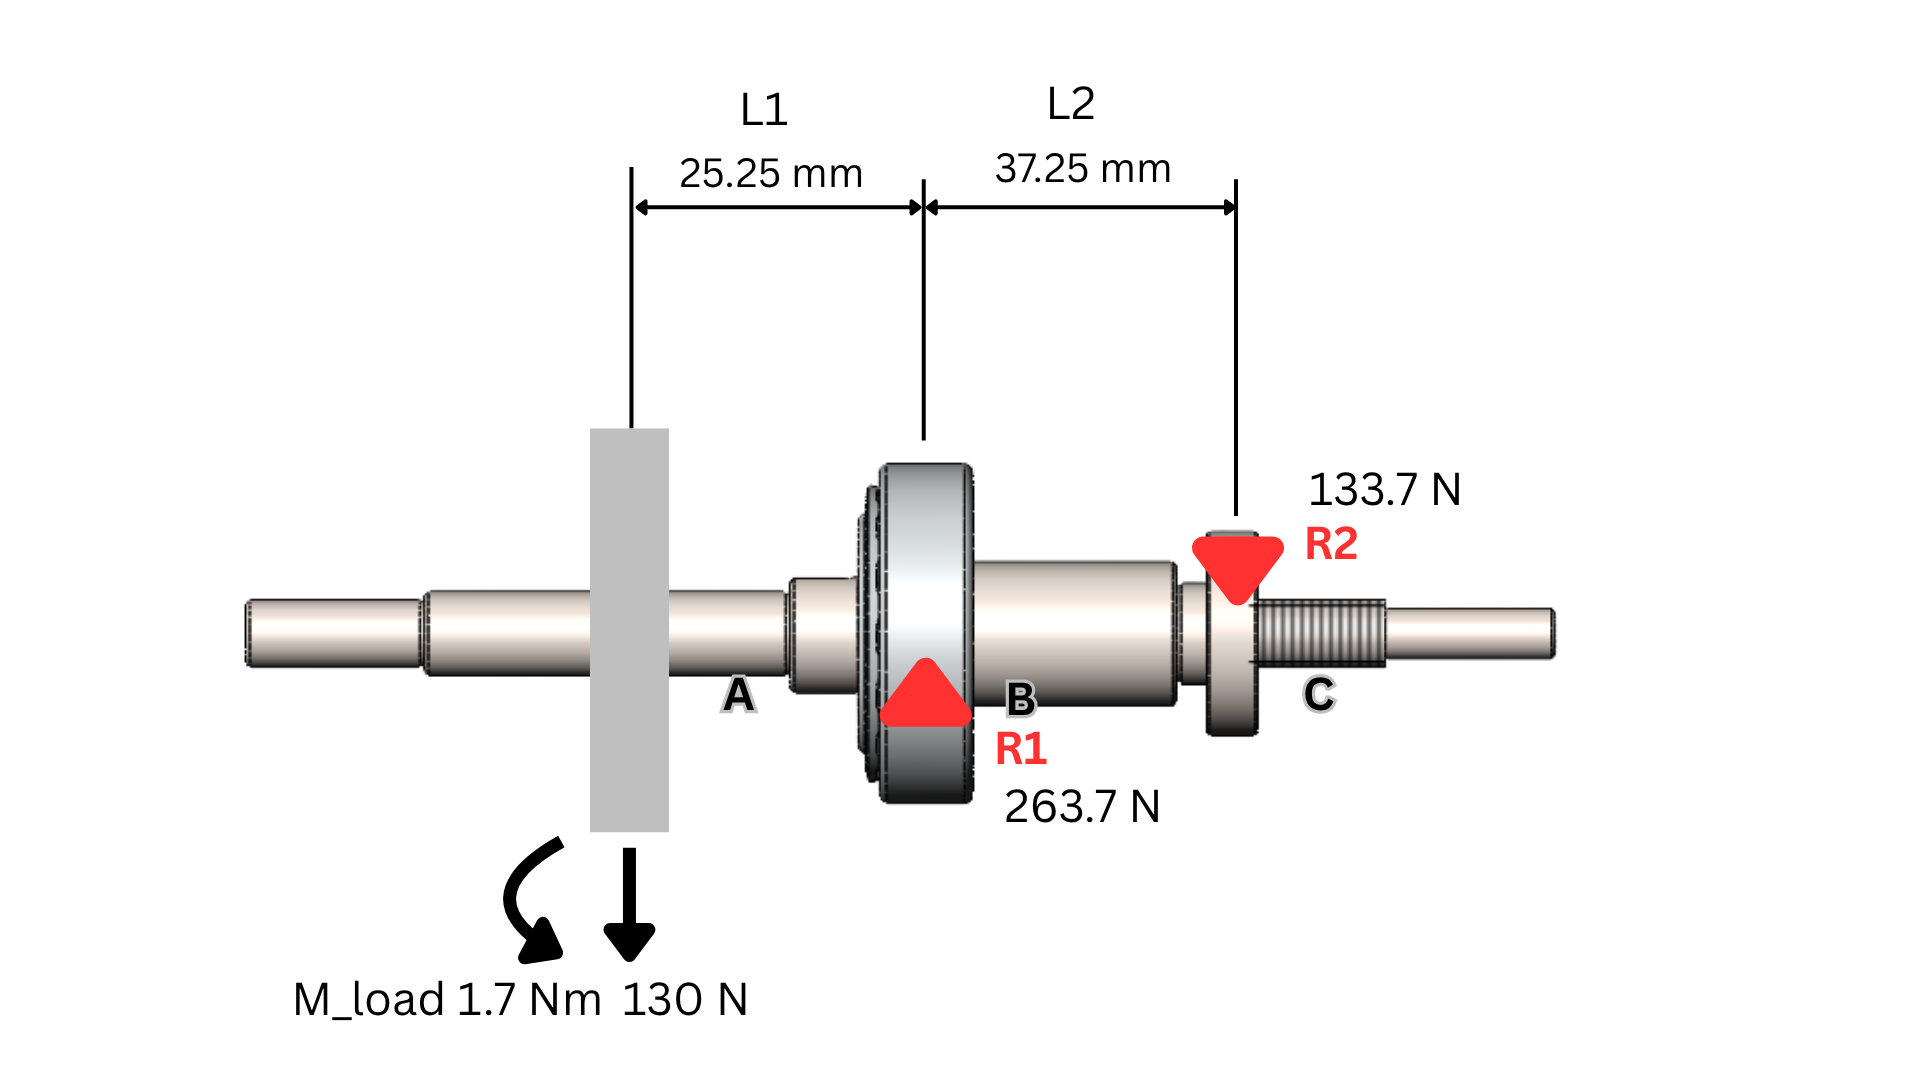
\includegraphics[width=0.7\textwidth]{images/FBDshaft.png}
    \caption{แผนภาพแสดงแรงกระทำและตำแหน่งของตลับลูกปืนบนเพลา}
    \label{fig:bearing_load_diagram}
\end{figure}

\textbf{รายละเอียดตลับลูกปืนแต่ละตำแหน่ง}
\begin{itemize}
    \item \textbf{ตลับลูกปืนเม็ดเรียว (Taper Roller Bearing - SKF 30203):} ใช้เป็นตลับลูกปืนหลักในการรับแรงดึงสายพานและโมเมนต์ดัด มีพิกัดการรับน้ำหนักพลวัต $C = 23.4$ kN จากการวิเคราะห์พบว่าอัตราส่วนแรง $F_a/F_r < e$ ($0.14 < 0.35$) ทำให้ได้ค่า Equivalent Load $P = 0.26$ kN คำนวณอายุการใช้งานได้ประมาณ $6.1 \times 10^8$ ชั่วโมง
    \item \textbf{ตลับลูกปืนเม็ดกลมร่องลึก (Deep Groove Ball Bearing - F6901ZZ):} ใช้เป็นตลับลูกปืนประคอง (Secondary Support) มีพิกัดการรับน้ำหนักพลวัต $C = 2.886$ kN และมีแรงสมมูลที่กระทำต่อตลับลูกปืนจุดนี้ $P = 0.1388$ kN คำนวณอายุการใช้งานได้ประมาณ $1.76 \times 10^6$ ชั่วโมง
\end{itemize}

\begin{table}[H]
    \centering
    \caption{สรุปผลการคำนวณภาระและอายุการใช้งานของตลับลูกปืน}
    \label{tab:bearing_life}
    \begin{tabular}{lcccc}
        \toprule
        \textbf{ตำแหน่ง / รุ่นตลับลูกปืน} & \textbf{$C$ (kN)} & \textbf{$P$ (kN)} & \textbf{$L_{10h}$ (Hours)} & \textbf{ผลการประเมิน} \\
        \midrule
        SKF 30203 (Taper Roller) & 23.400 & 0.2600 & $6.1 \times 10^8$ & \textbf{ผ่าน} \\
        F6901ZZ (Deep Groove Ball) & 2.886 & 0.1388 & $1.76 \times 10^6$ & \textbf{ผ่าน} \\
        \bottomrule
    \end{tabular}
\end{table}

\textbf{สรุปผลการประเมิน} จากการเปรียบเทียบกับเกณฑ์มาตรฐานการออกแบบเครื่องจักรกลทั่วไปที่มักกำหนดเป้าหมายอายุการใช้งานไว้ที่ 20,000 – 100,000 ชั่วโมง \citep{skf_bearing} พบว่าตลับลูกปืนทั้งสองตำแหน่งที่เลือกใช้มีอายุการใช้งานทางทฤษฎีสูงกว่าเกณฑ์ขั้นต่ำอย่างมีนัยสำคัญ จึงมีความเหมาะสมในการใช้งานภายใต้สภาวะโหลดที่กำหนด \citep{skf_bearing}

%--------------------------------------------------------------------------------------------------------------------------

% ----------------------------------------------------------------------------
% การวิเคราะห์การโก่งตัว (Deflection Analysis)
% ----------------------------------------------------------------------------
\subsection{การวิเคราะห์การโก่งตัว (Deflection Analysis)}
\label{subsec:deflection_analysis}

\subsubsection{ผล FEA และการคํานวณ Deflection (ภายใต้ โหลด 2.7 kg)}
\label{subsubsec:fea_deflection_calculation}

\textbf{ก. ข้อมูลเริ่มต้นและสภาวะการทดสอบ (Test Conditions \& Parameters)}
\begin{itemize}
    \item \textbf{แรงกระทำ (Applied Load):} ใช้วัตถุที่มีน้ำหนักรวม 2.7 kg (คิดเป็นแรงกระทำประมาณ $F = mg = 2.7 \times 9.81 = 26.487$ N)
    \item \textbf{วัสดุที่ใช้ในการทดสอบ:} แป๊บโปร่งกัลวาไนซ์ (Galvanized Square Pipe) มาตรฐาน มอก. ขนาด 25 x 25 มม. ความหนา 2.3 มม.
    \item \textbf{ลักษณะจุดรองรับ (Boundary Conditions):} ทำการยึดฐานของหุ่นยนต์เข้ากับหน้าโต๊ะด้วยอุปกรณ์ C-Clamp (เสมือนจุดรองรับแบบยึดแน่น หรือ Fixed Support) โดยให้ Load กดลงที่บริเวณปลายแขนของหุ่นยนต์ ทั้งนี้ได้มีการเผื่อระยะพื้นที่บริเวณปลายแขนสำหรับติดตั้งไดอัลเกจ (Dial Gauge) เพื่อทำการวัดค่า
\end{itemize}

\textbf{ข. ผลการวิเคราะห์ด้วยโปรแกรม (FEA Simulation Results)}

\begin{figure}[H]
    \centering
    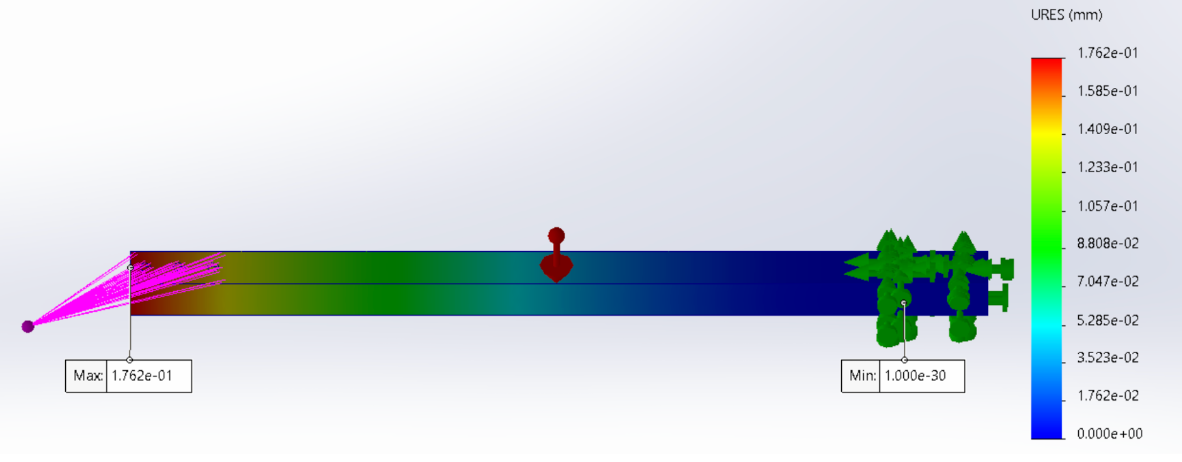
\includegraphics[width=0.8\textwidth]{images/ArmFEA.png}
    \caption{แสดงการทำ FEA ใส่โหลดที่ 2.7 kg}
    \label{fig:fea_deflection_2_7kg}
\end{figure}

ดำเนินการวิเคราะห์แบบ Static Study ผ่านโปรแกรม SOLIDWORKS Simulation เพื่อตรวจสอบความแข็งแรงและการโก่งตัวภายใต้เกณฑ์โหลดสูงสุด 2 kg (ตามข้อกำหนด M3) และทดสอบที่โหลดอ้างอิง 2.76 kg 

\textbf{ผลลัพธ์ที่ได้:} 
\begin{itemize}
    \item จากผลการวิเคราะห์พบว่าระยะการโก่งตัวสูงสุด ($\delta_{max}$) คือ 0.2281 mm โดยเกิดการโก่งตัวมากที่สุดบริเวณปลายแขนที่รับภาระกรรม
    \item ค่าความเค้น Von Mises สูงสุดอยู่ที่ $2.131 \times 10^7$ N/m$^2$ ซึ่งคิดเป็นเพียง 9.1\% ของ Yield Strength ($2.35 \times 10^8$ N/m$^2$)
    \item ค่า Factor of Safety ต่ำสุดเท่ากับ 11.03 ซึ่งสูงกว่าเกณฑ์ขั้นต่ำอย่างปลอดภัย 
\end{itemize}
สรุปได้ว่าโครงสร้างสามารถรับโหลดได้อย่างปลอดภัยตามข้อกำหนด

\textbf{ค. ผลการทดสอบการโก่งตัวจากชิ้นงานจริง (Experimental Results with 2.7 kg Load)}

\textbf{วิธีการวัด:} ติดตั้งหัววัดของไดอัลเกจ (Dial Gauge) ให้สัมผัสกับตำแหน่งปลายสุดของแขนหุ่นยนต์ จากนั้นทำการเซ็ตศูนย์ (Set Zero) ที่มาตรวัด นำวัตถุน้ำหนัก 2.7 kg มากระทำที่ปลายแขนหุ่นยนต์ แล้วจึงอ่านค่าระยะการโก่งตัวที่เปลี่ยนไปจากหน้าปัดของไดอัลเกจ

\begin{figure}[H]
    \centering
    \begin{subfigure}{0.45\textwidth}
        \centering
        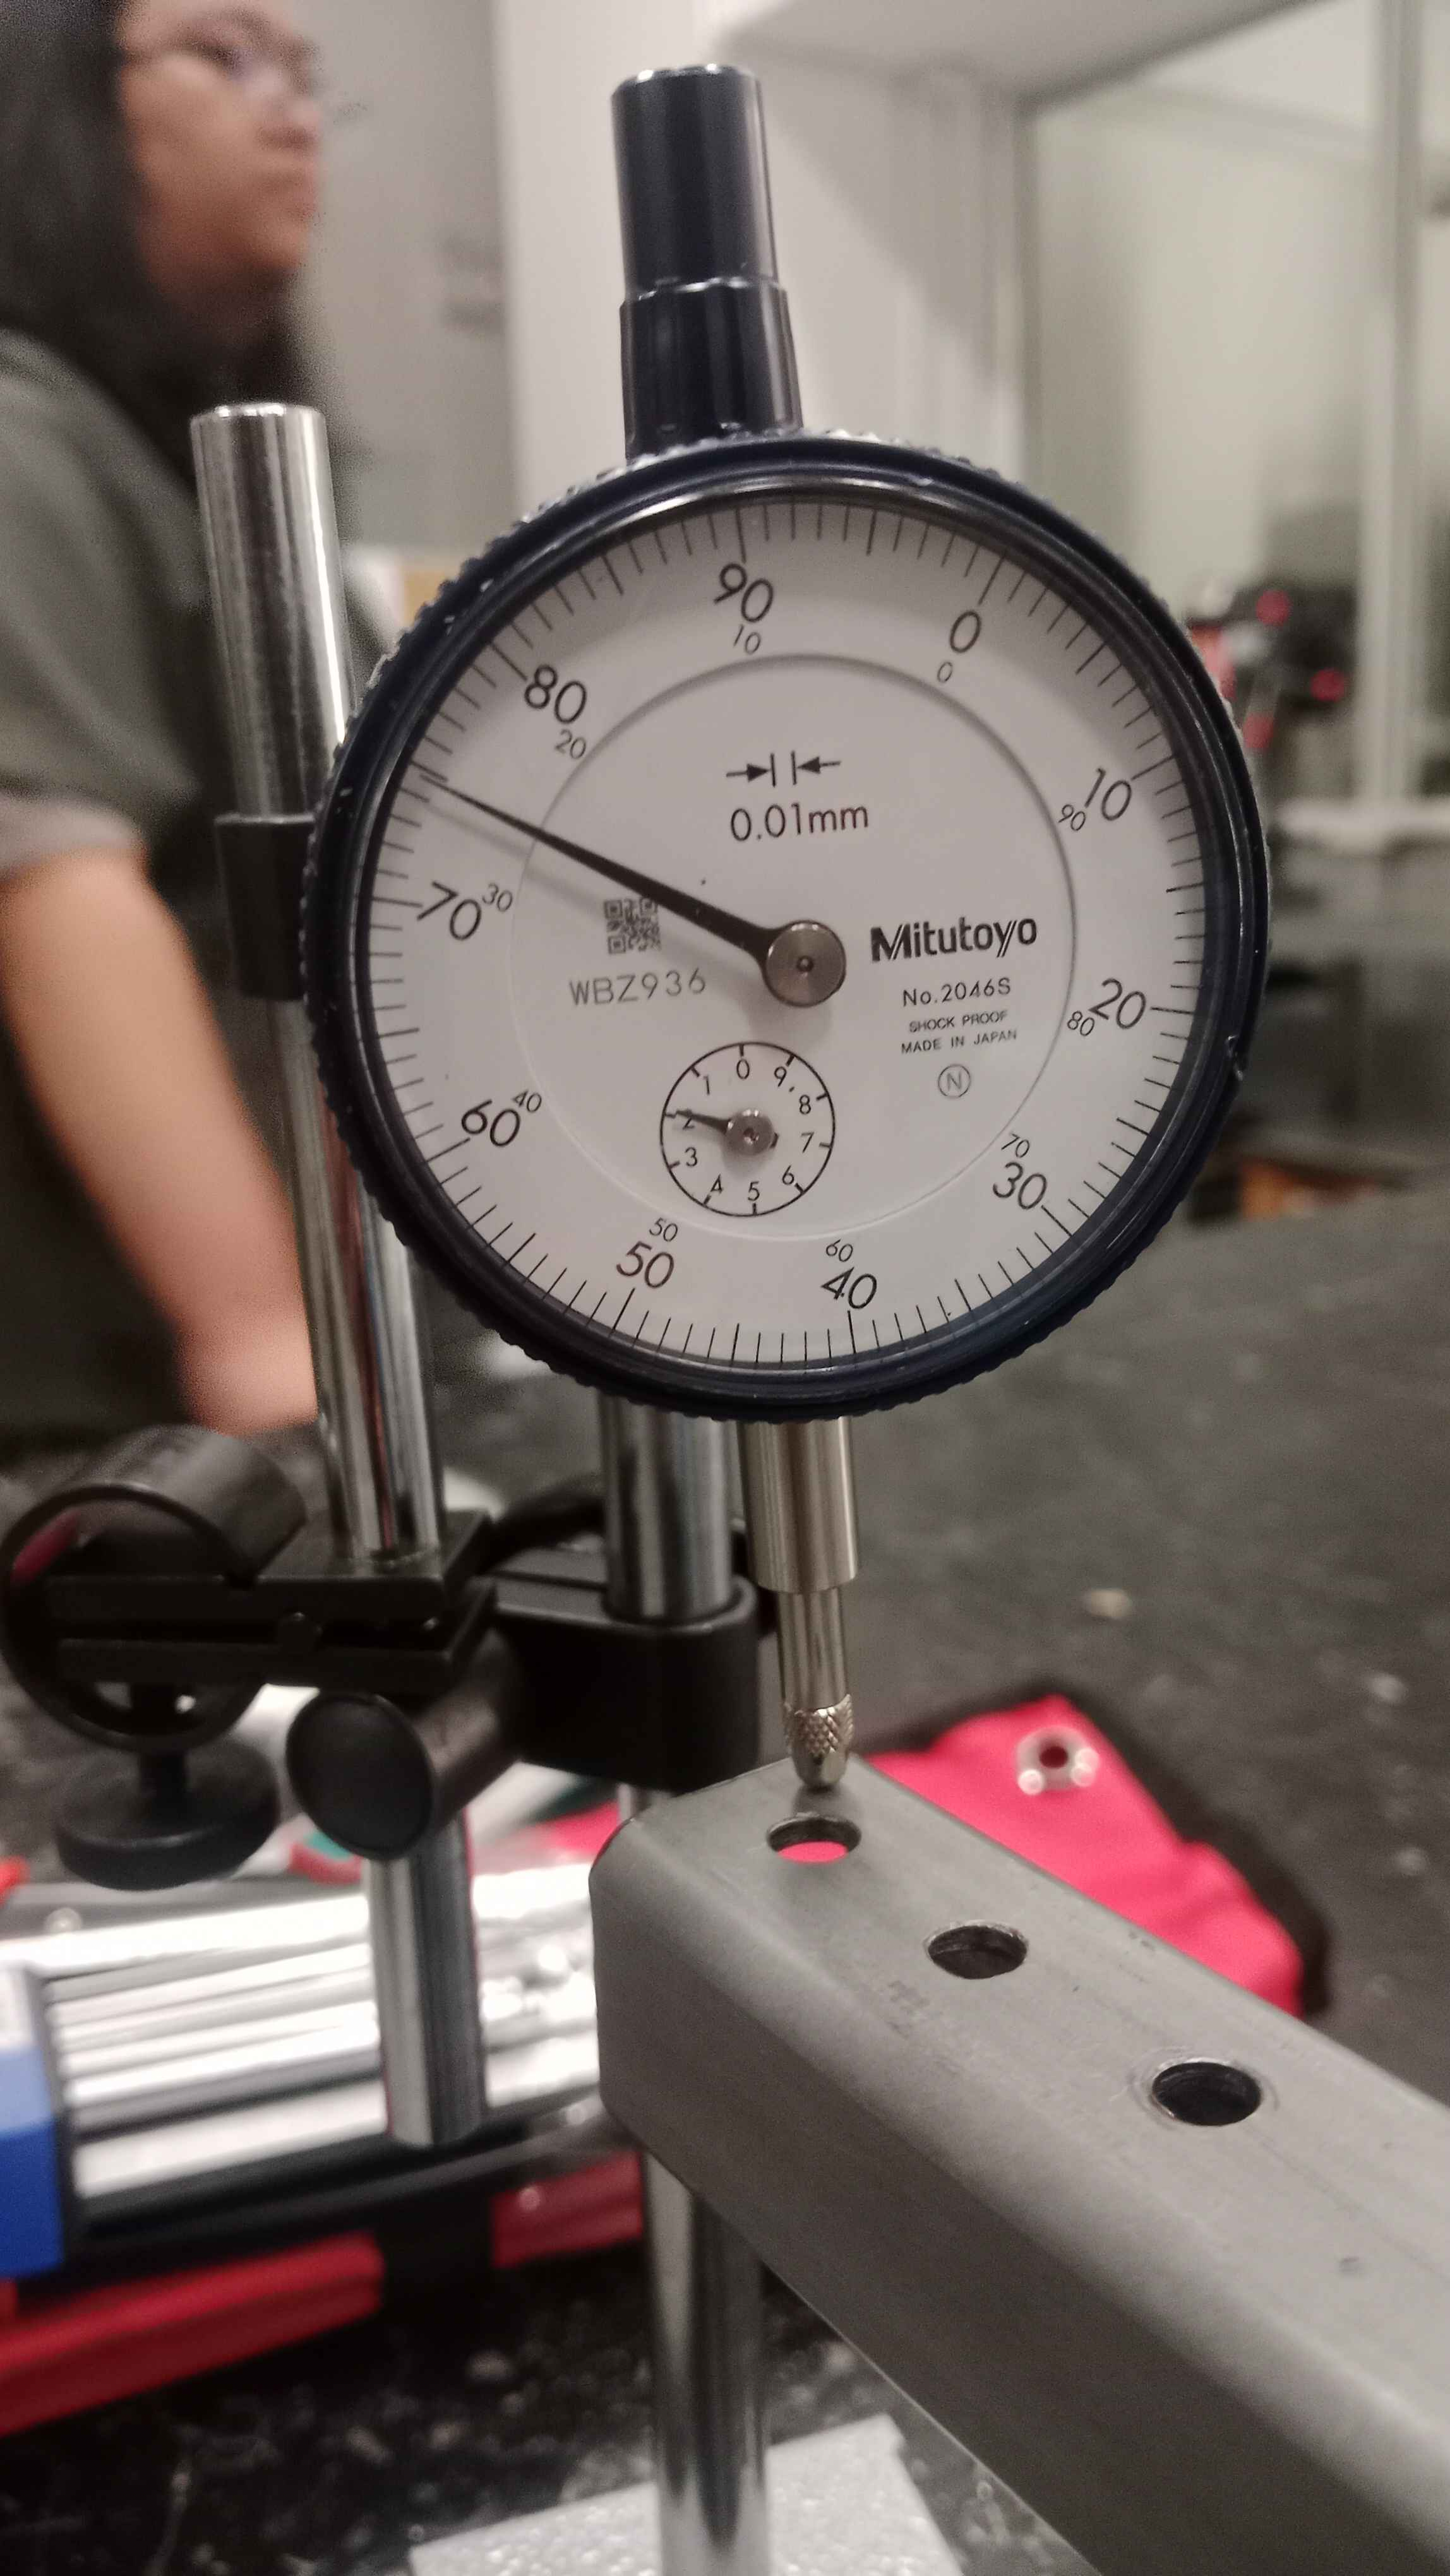
\includegraphics[width=\textwidth]{images/Deflection_1.jpg}
        \caption{ตำแหน่งที่ใช้ Dial Gauge บนโครงสร้างชิ้นงานจริง}
        \label{fig:dial_gauge_setup}
    \end{subfigure}
    \hfill
    \begin{subfigure}{0.45\textwidth}
        \centering
        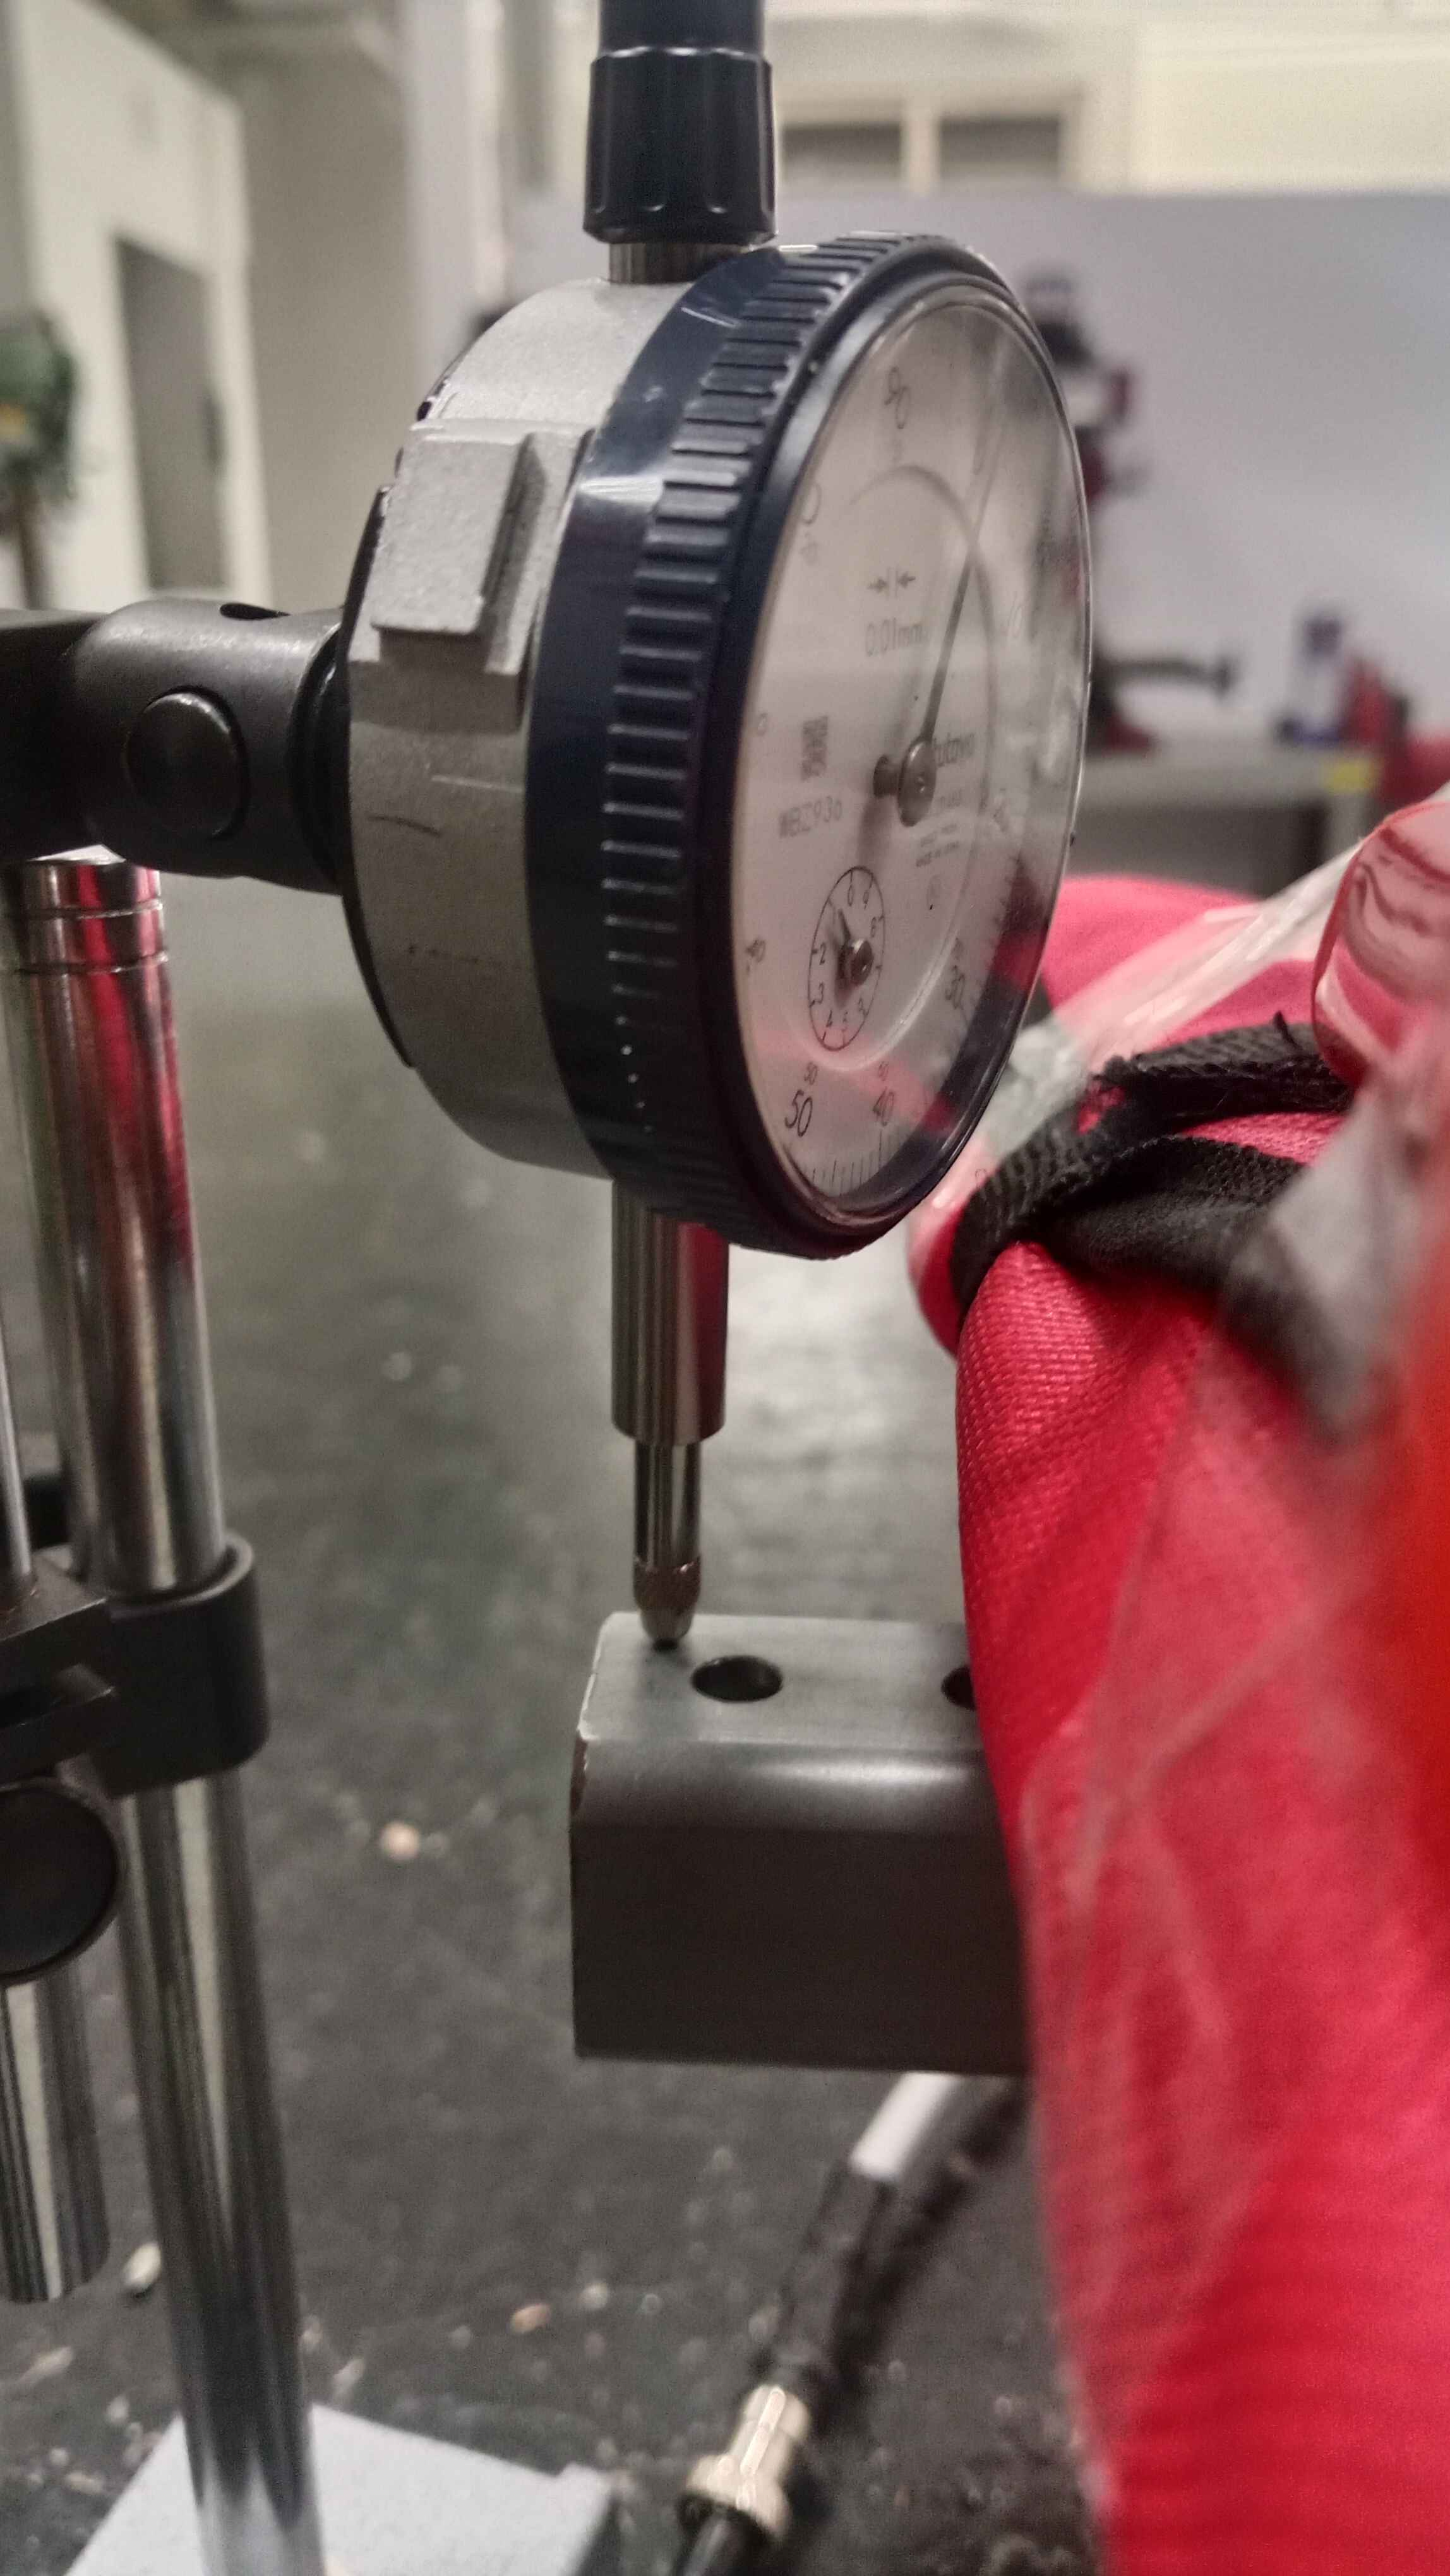
\includegraphics[width=\textwidth]{images/Deflection_2.jpg}
        \caption{หน้าปัดมาตรวัดแสดงระยะโก่งตัว}
        \label{fig:dial_gauge_reading}
    \end{subfigure}
    \caption{การทดสอบการโก่งตัวทางกลด้วย Dial Gauge}
    \label{fig:dial_gauge_test}
\end{figure}

\textbf{ผลการทดสอบ:} จากการทดสอบจริง พบว่าระยะการโก่งตัว (Deflection) ที่วัดได้จากชิ้นงานมีค่าอยู่ที่ 0.75 mm

\textbf{ง. การคำนวณองศาการบิดเบี้ยวของปลายแขนหุ่น (Deflection Angle Calculation)}

เพื่อประเมินว่าปลายแขนของหุ่นยนต์ทำมุมเบี่ยงเบนไปจากแนวระนาบเดิมเท่าใด สามารถคำนวณองศาที่เบี้ยวไป ($\theta$) ได้จากหลักการทางตรีโกณมิติ โดยใช้ระยะการโก่งตัวที่วัดได้จริง ($\delta = 0.75$ mm) และระยะความยาวของแขนหุ่นยนต์ ($L = 403.1$ mm) วัดจากจุดหมุนจนถึงปลายตำแหน่งที่วัดค่าตามสมการที่ \ref{eq:deflection_angle}
\begin{equation}
    \theta = \arctan \left( \frac{\delta}{L} \right)
    \label{eq:deflection_angle}
\end{equation}

ตัวอย่างการคำนวณ:
\begin{figure}[H]
    \centering
    \begin{subfigure}{0.48\textwidth}
        \centering
        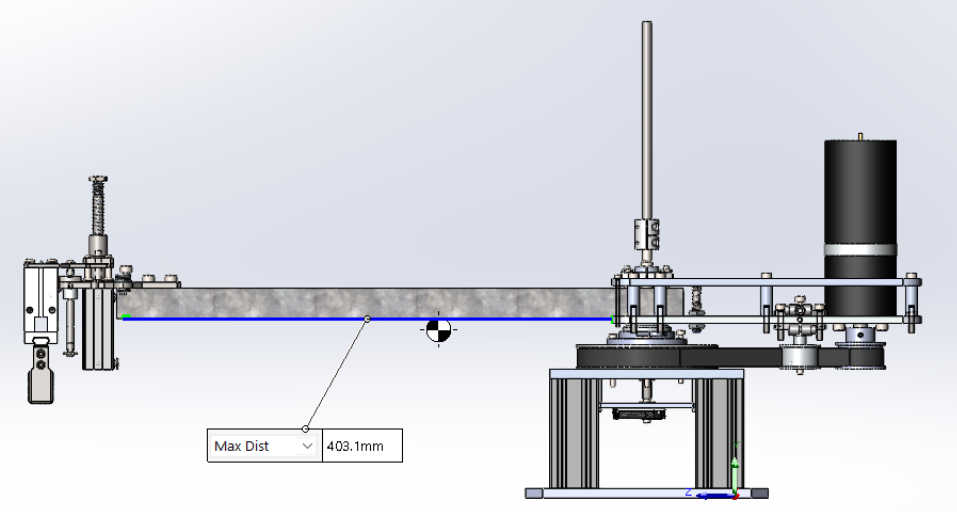
\includegraphics[width=\textwidth]{images/Armlength.png}
        \caption{แสดงระยะจากจุดหมุนถึงปลายแขนรับน้ำหนัก}
        \label{fig:arm_length_cad}
    \end{subfigure}
    \hfill
    \begin{subfigure}{0.48\textwidth}
        \centering
        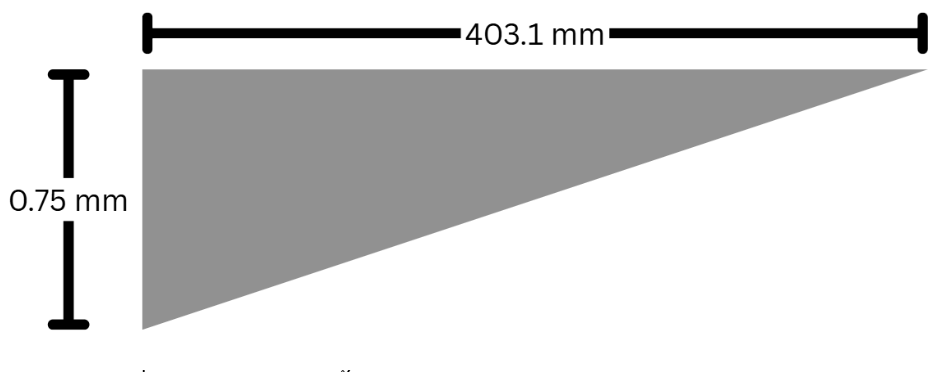
\includegraphics[width=\textwidth]{images/Trigonometry.png}
        \caption{สามเหลี่ยมตรีโกณมิติแสดงมุมเบี่ยงเบนเชิงมุม}
        \label{fig:deflection_triangle}
    \end{subfigure}
    \caption{การวิเคราะห์ระยะและมิติเชิงเรขาคณิตเพื่อคำนวณมุมบิดเบี้ยว}
    \label{fig:deflection_geometry_analysis}
\end{figure}

\begin{equation}
    \theta = \arctan \left( \frac{0.75}{403.1} \right) = 0.1066^\circ
\end{equation}

\textbf{สรุปผล:} ปลายแขนหุ่นยนต์มีมุมบิดเบี้ยวเบี่ยงเบนไปจากแนวระนาบประมาณ $0.1066^\circ$ 

\textbf{จ. การเปรียบเทียบผลลัพธ์และการวิเคราะห์ (Comparison \& Discussion)}

\begin{table}[H]
    \centering
    \caption{เปรียบเทียบค่าการโก่งตัวและเปอร์เซ็นต์ความคลาดเคลื่อนภายใต้แรง 2.7 kg}
    \label{tab:deflection_comparison}
    \begin{tabular}{lcc}
        \toprule
        \textbf{วิธีการประเมินผล} & \textbf{ระยะการโก่งตัว (mm)} & \textbf{ความคลาดเคลื่อน (\% Error)} \\
        \midrule
        การวิเคราะห์ด้วย FEA (Simulation) & 0.2281 & 69.58\% \\
        การทดสอบจากชิ้นงานจริง (Experiment) & 0.75 & 0.00\% (ค่าอ้างอิง) \\
        \bottomrule
    \end{tabular}
\end{table}

สูตรคำนวณความคลาดเคลื่อนเทียบจากการทดลองจริงคือสมการที่ \ref{eq:error_calc} และคำนวณได้ดังสมการที่ \ref{eq:error_result}
\begin{equation}
    \% \text{ Error} = \frac{|\text{Real} - \text{FEA}|}{\text{Real}} \times 100 
    \label{eq:error_calc}
\end{equation}
\begin{equation}
    \% \text{ Error} = \frac{|0.75 - 0.2281|}{0.75} \times 100 = 69.58\%
    \label{eq:error_result}
\end{equation}

\textbf{การอภิปรายผล (Discussion):}
จากตารางที่ \ref{tab:deflection_comparison} พบว่าระยะการโก่งตัวจากการทดสอบจริง (0.75 mm) มีค่ามากกว่าผลที่ได้จากการจำลองด้วย FEA (0.2281 mm) อย่างมีนัยสำคัญ โดยมีความคลาดเคลื่อนอยู่ที่ 69.58\% ซึ่งสามารถวิเคราะห์สาเหตุของความแตกต่างนี้ได้จากปัจจัยต่างๆ ดังนี้:
\begin{itemize}
    \item \textbf{ลักษณะของจุดรองรับ (Boundary Condition Mismatch):} ในโปรแกรม FEA จุดรองรับถูกกำหนดให้เป็นแบบยึดแน่นสมบูรณ์ (Perfectly Fixed) แต่ในการทดลองจริง การยึดฐานด้วย C-Clamp อาจมีการให้ตัว (Flexibility) ได้เล็กน้อยเมื่อรับแรงกระทำ ทำให้เกิดมุมเงยหรือการบิดตัวที่ฐาน ซึ่งส่งผลขยายให้ระยะแอ่นตัวที่ปลายแขนมีค่ามากขึ้น
    \item \textbf{ความคลาดเคลื่อนของรอยต่อและข้อต่อ:} หากแขนหุ่นยนต์มีการประกอบหรือมีรอยเชื่อม/ข้อต่อ ความหลวม (Backlash) หรือช่องว่างในจุดหมุนเหล่านั้นจะบวกเพิ่มเข้าไปในระยะโก่งตัวจริง ซึ่งโปรแกรม FEA (ที่วิเคราะห์แบบชิ้นเนื้อเดียวติดกันสมบูรณ์) ไม่ได้นำมาคำนวณรวมด้วย
    \item \textbf{น้ำหนักของโครงสร้าง (Self-weight):} ในขั้นตอนการเซ็ตศูนย์ (Set Zero) ของการทดลองจริง ภาระกรรมของน้ำหนักแขนหุ่นยนต์อาจมีผลต่อการกระจายแรงเมื่อได้รับน้ำหนักเพิ่ม หรือความเค้นตกค้างในวัสดุ
    \item \textbf{ความแม่นยำของเครื่องมือวัด:} แม้ไดอัลเกจจะมีความละเอียดสูง แต่ตำแหน่งจุดสัมผัส มุมในการตั้งเกจ หรือความสั่นสะเทือนขณะวางน้ำหนักทดสอบ อาจส่งผลให้ค่าที่อ่านได้มีความคลาดเคลื่อนจากการกระจัดเชิงเส้นแบบอุดมคติในโปรแกรม
    \item \textbf{ความแตกต่างของจุดศูนย์กลางมวล (Center of Mass Discrepancy):} ในโปรแกรม FEA ภาระกรรม 2.7 kg มักถูกกำหนดให้กระทำลงบนตำแหน่งที่เจาะจงหรือมีจุดศูนย์กลางมวล (Center of Mass) ที่แม่นยำ (เช่น แรงกระทำแบบจุด หรือ Point Load) แต่ในการทดลองจริง วัตถุที่นำมาใช้เป็นน้ำหนักมีรูปทรง ขนาด และการกระจายน้ำหนักที่ต่างออกไป ทำให้ไม่สามารถจัดวางจุดศูนย์กลางมวลของวัตถุให้ตกลงบนตำแหน่งเดียวกับในแบบจำลองได้อย่างสมบูรณ์แบบ การเยื้องศูนย์ (Eccentricity) ของแนวแรงหรือแขนโมเมนต์ที่คลาดเคลื่อนไปเพียงเล็กน้อยนี้ จะส่งผลให้โมเมนต์ดัด (Bending Moment) ที่เกิดขึ้นจริงบนปลายแขนหุ่นยนต์มีค่าแตกต่างไปจากโปรแกรม และทำให้เกิดระยะการโก่งตัวที่มากขึ้นได้
\end{itemize}

% ----------------------------------------------------------------------------
% การวิเคราะห์ระยะคลอน (Backlash Analysis)
% ----------------------------------------------------------------------------
\subsection{การวิเคราะห์ระยะคลอน (Backlash Analysis)}
\label{subsec:backlash_analysis}

\begin{figure}[H]
    \centering
    \begin{subfigure}{0.48\textwidth}
        \centering
        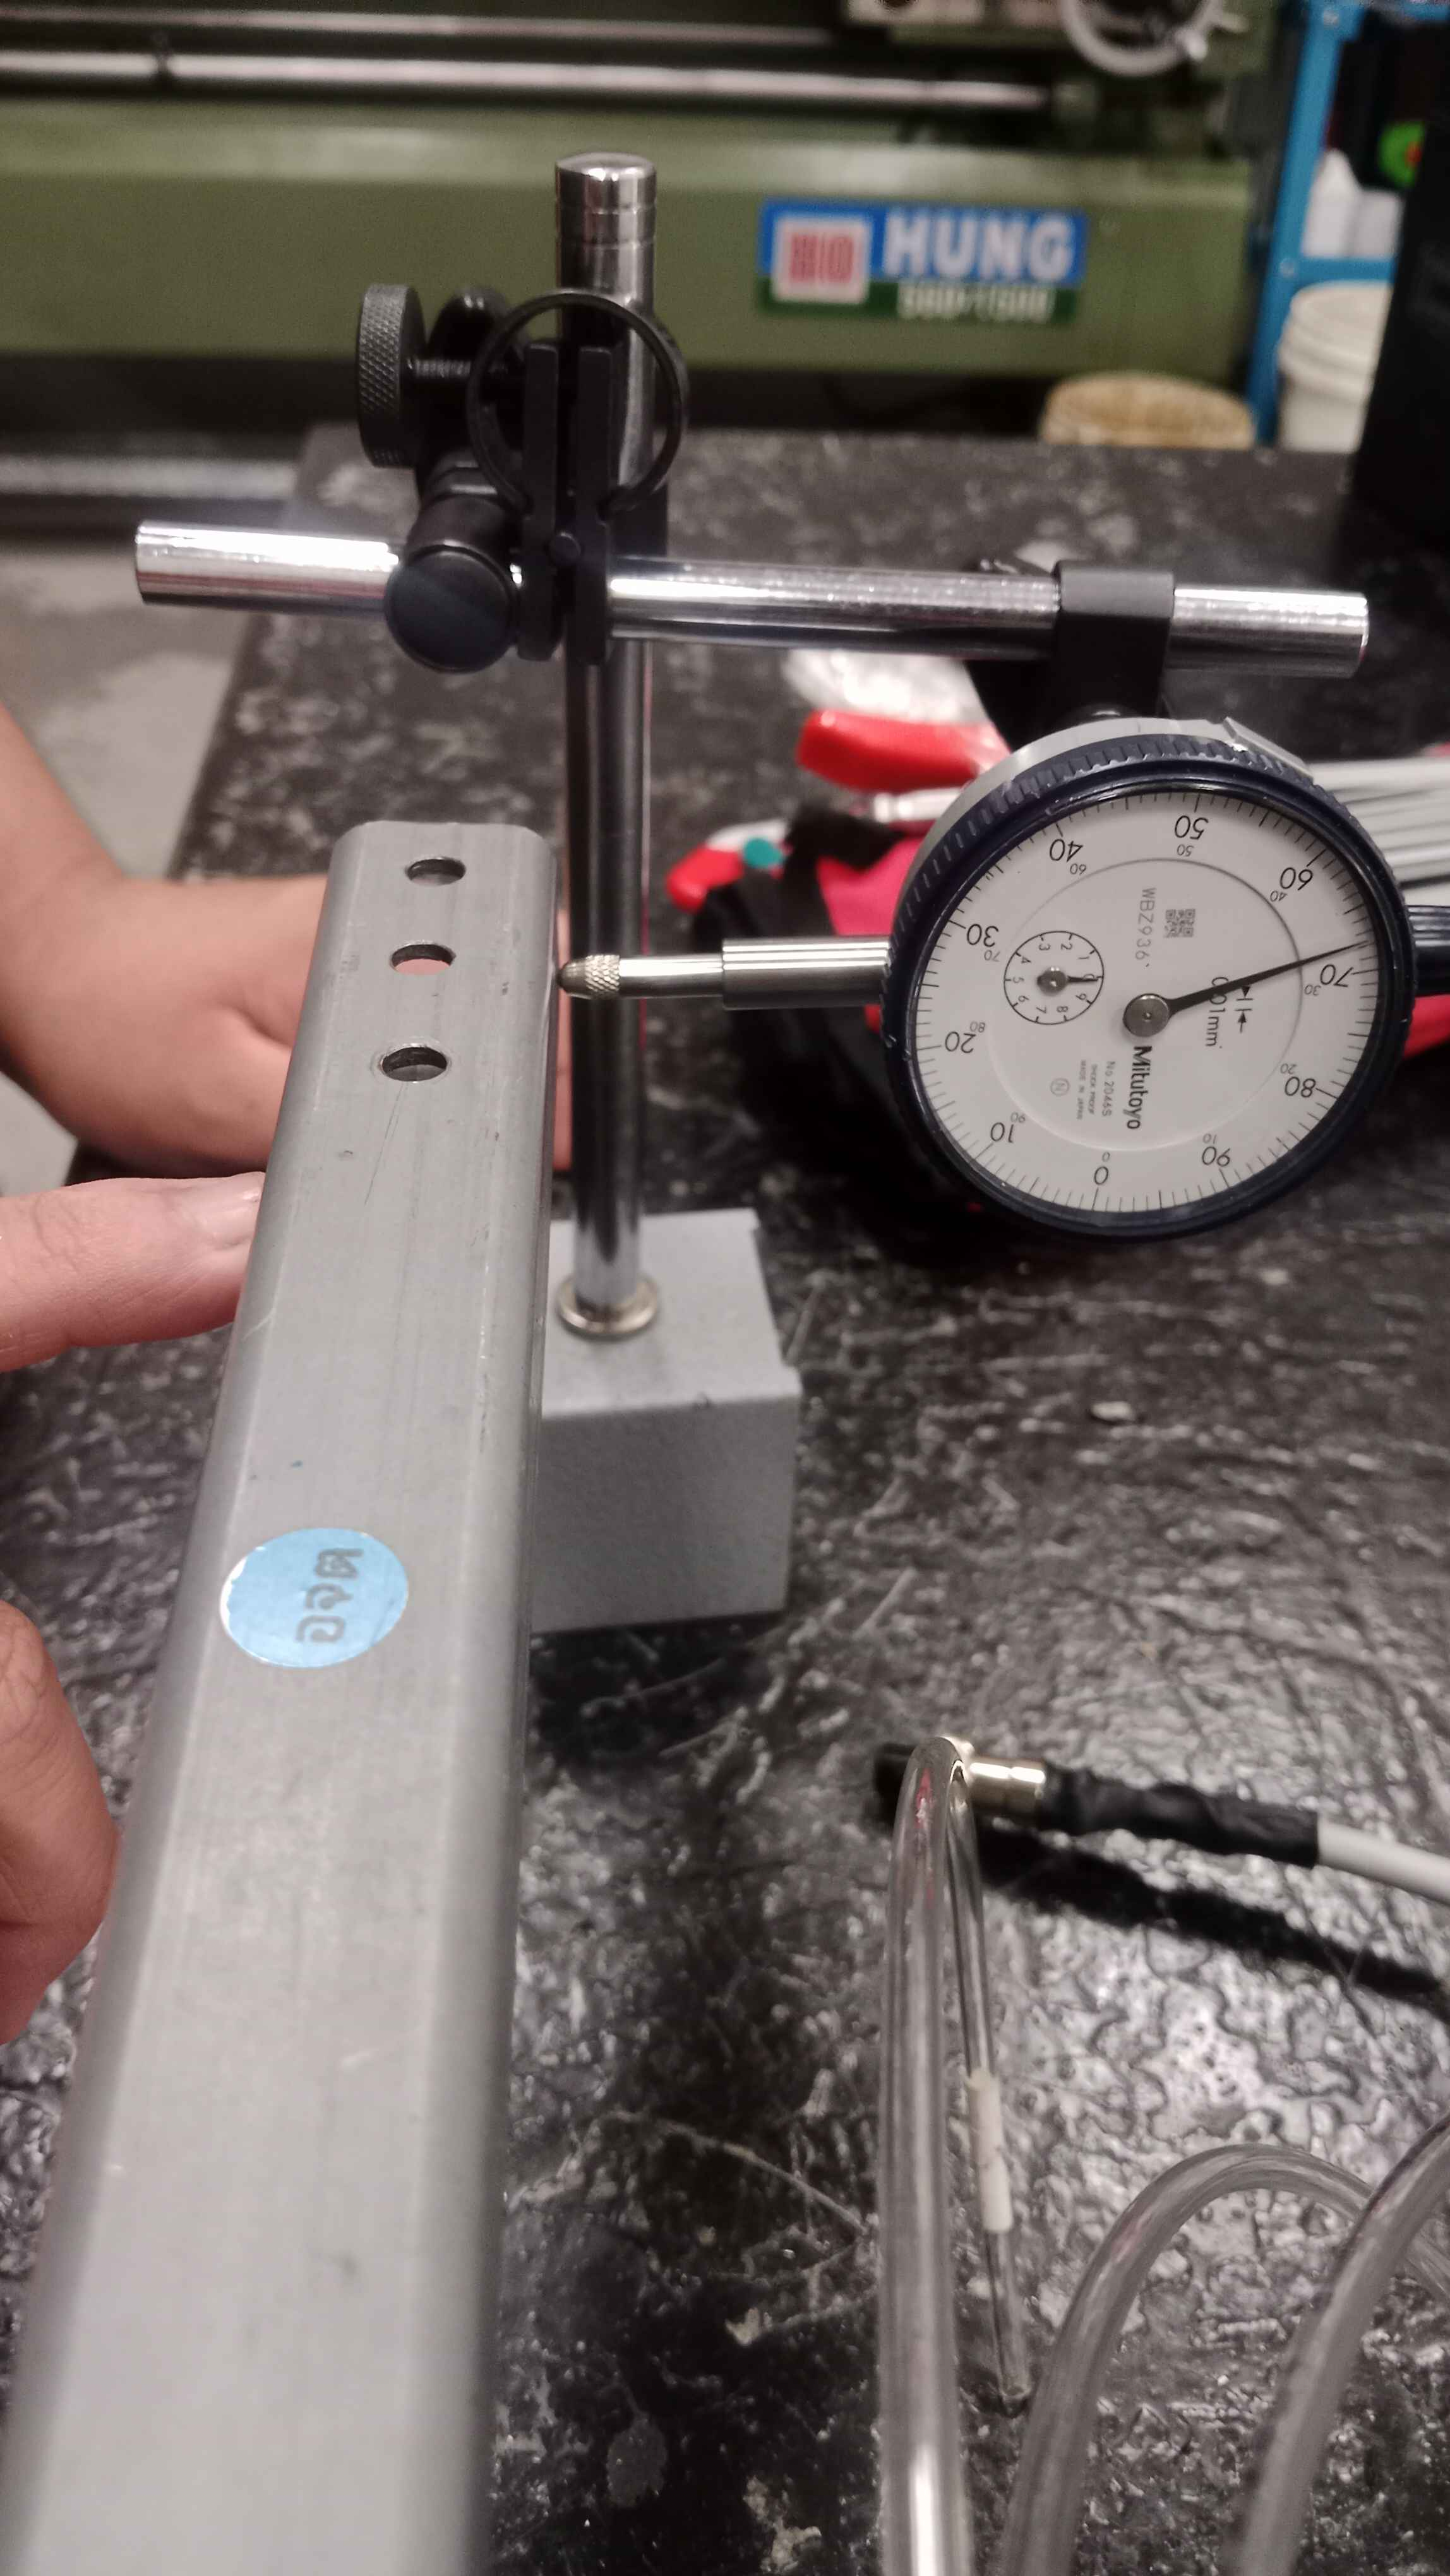
\includegraphics[width=\textwidth]{images/Backlash_1.jpg}
        \caption{การติดตั้งหัววัด Dial Gauge}
        \label{fig:backlash_setup_1}
    \end{subfigure}
    \hfill
    \begin{subfigure}{0.48\textwidth}
        \centering
        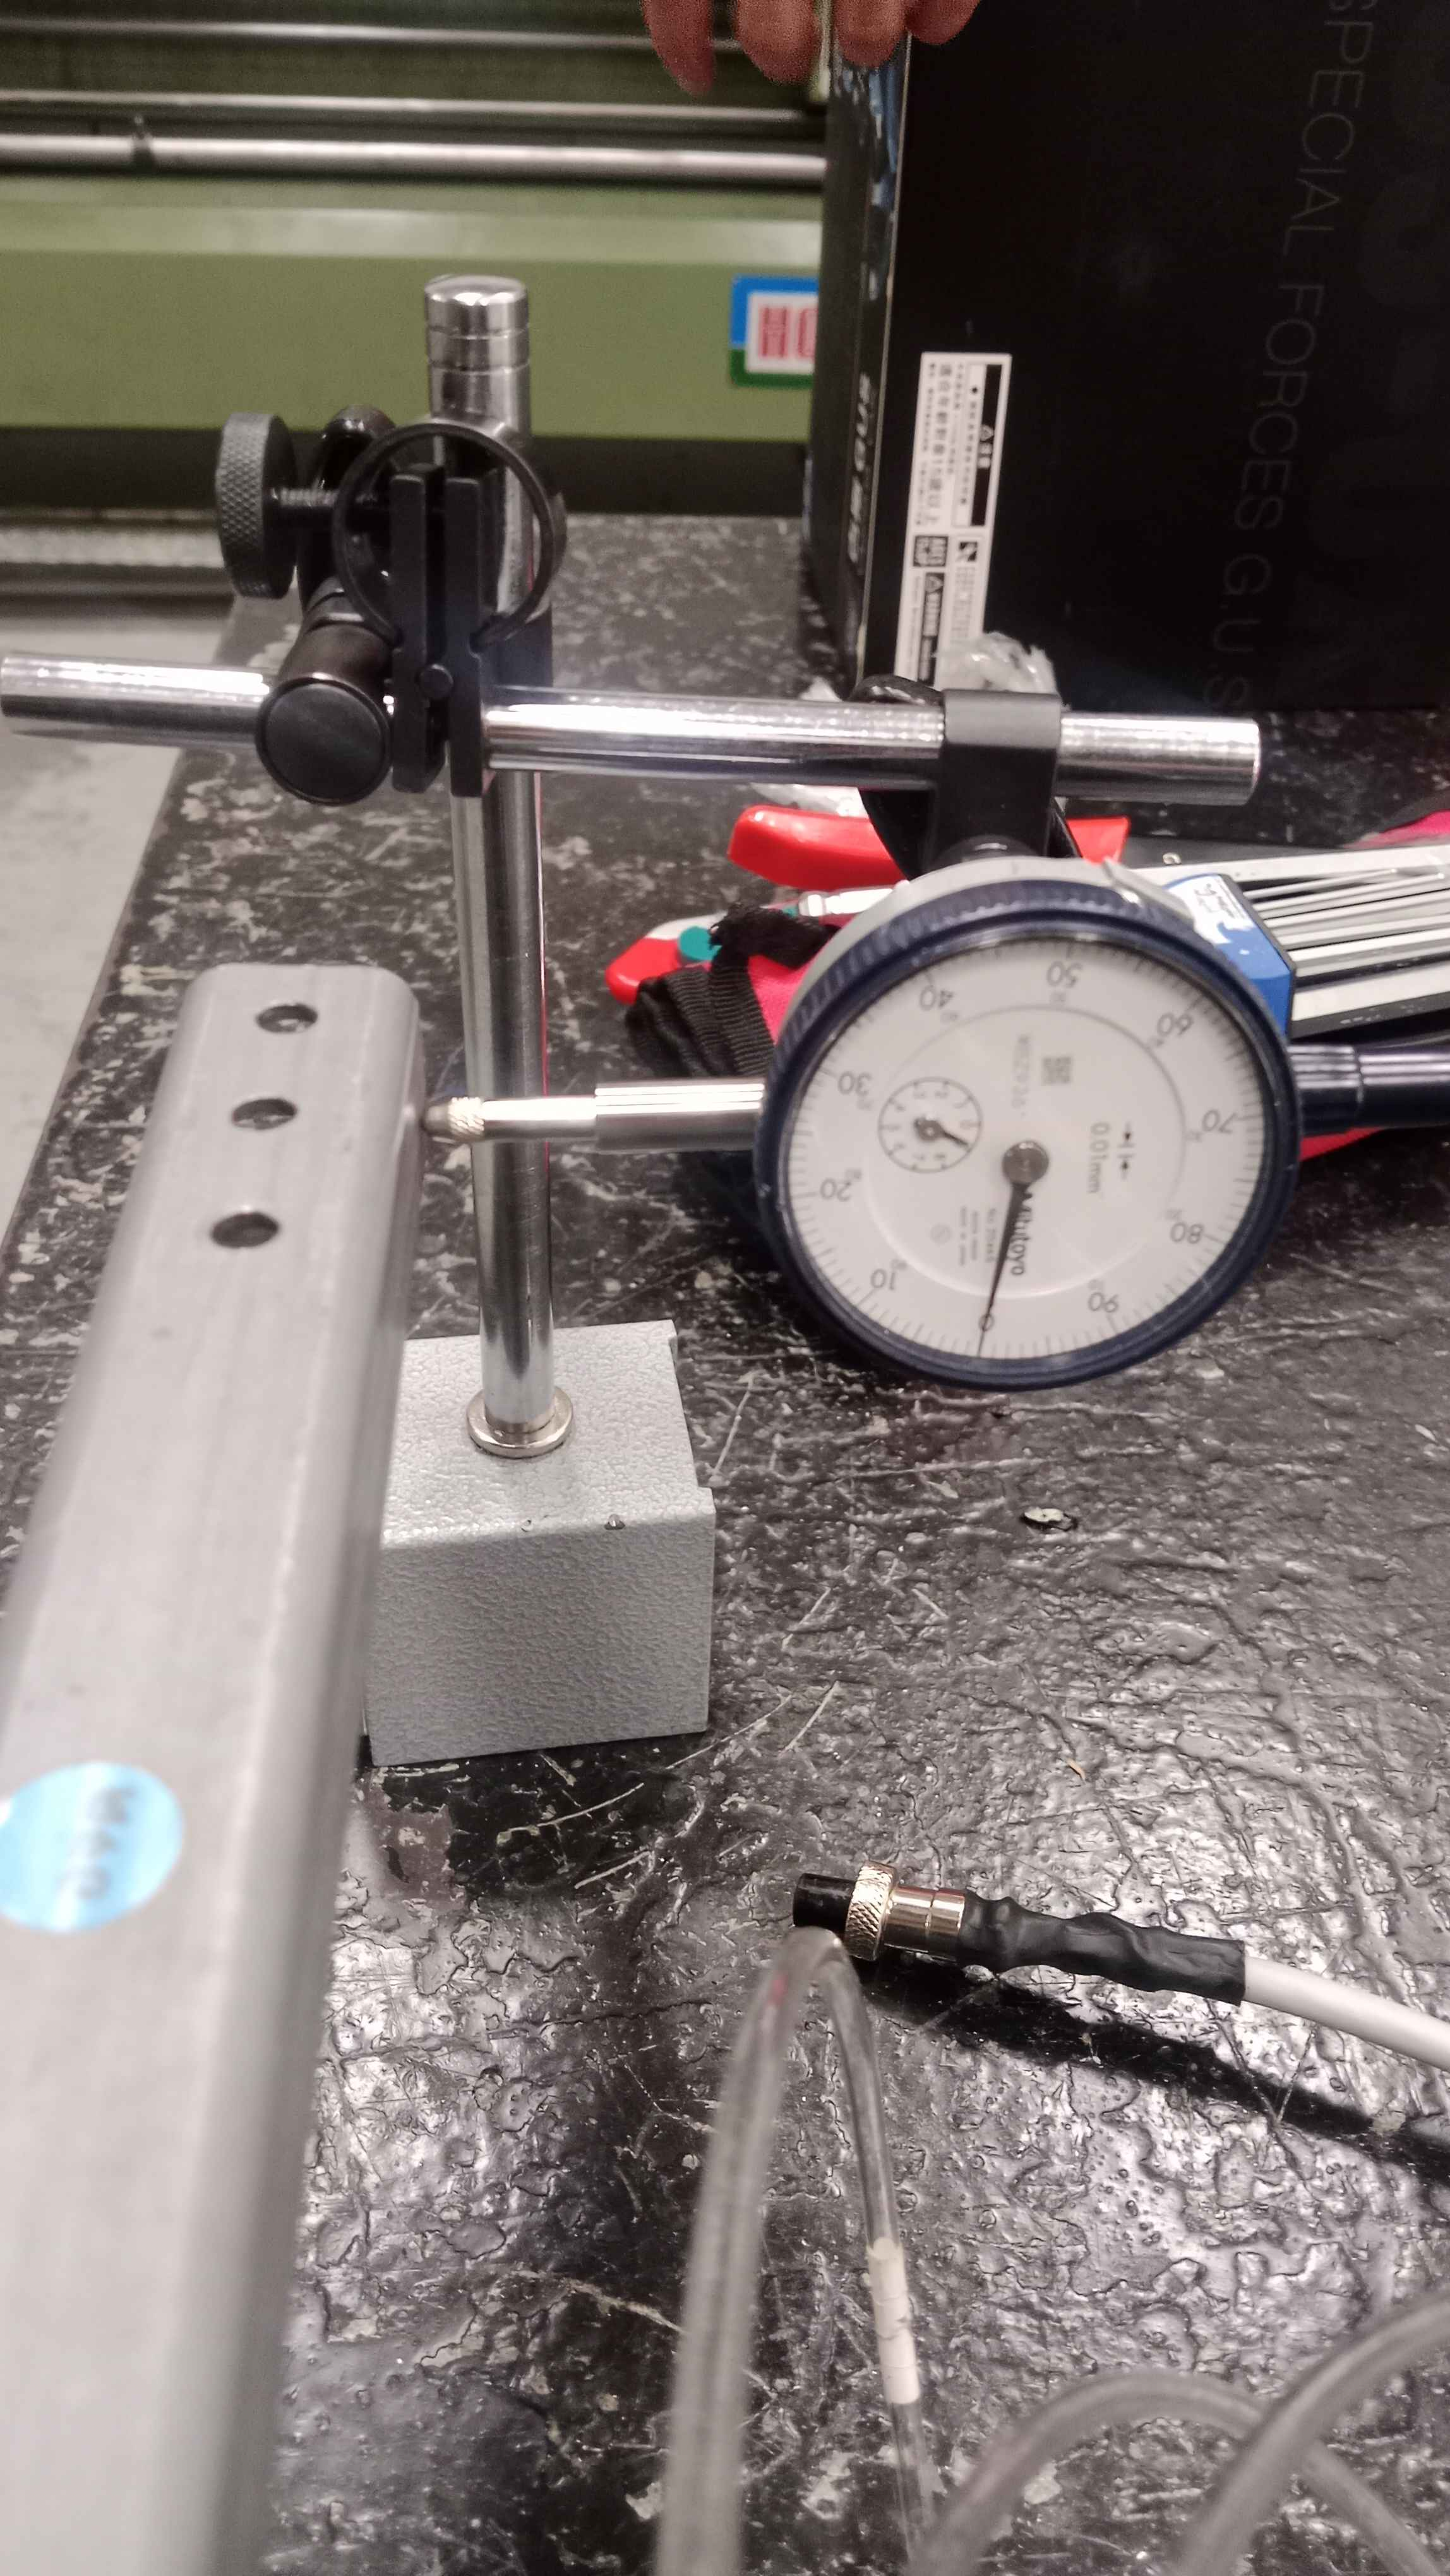
\includegraphics[width=\textwidth]{images/Backlash_2.jpg}
        \caption{ผลการอ่านค่าเมื่อออกแรงดัน}
        \label{fig:backlash_setup_2}
    \end{subfigure}
    \caption{การทดสอบระยะคลอนด้วย Dial Gauge}
    \label{fig:backlash_test_figure}
\end{figure}

ทดสอบโดยใช้เครื่องมือ Dial Gauge แล้วลองดันให้เกิด Backlash พบว่า ระยะคลอนมีระยะ 0.7 mm


% ============================================================
\subsection{การออกแบบระบบไฟฟ้าและอิเล็กทรอนิกส์ (Electronics Design)}
\label{subsec:electronics_design}
% ============================================================

\subsubsection{สถาปัตยกรรมไฟฟ้าโดยรวม}
\label{subsubsec:electrical_architecture}

ระบบไฟฟ้าแบ่งออกเป็น 2 วงจรหลักที่แยกจากกันอย่างชัดเจน
เพื่อให้ระบบ E-Stop ตัดเฉพาะกำลังไฟของมอเตอร์
โดยที่ Controller ยังคงมีไฟเลี้ยงอยู่ตามข้อกำหนด E6

\textbf{วงจร High Power (24\,V Motor Bus):}
ไฟ AC 220\,V เข้ามาผ่าน Circuit Breaker CB1 แล้ว จ่ายให้ PSU 24\,V/10\,A Output ของ PSU ผ่าน NC Contact 
ของปุ่ม Emergency Stop แล้วต่อเข้า COM ของ Relay module เมื่อมีสัญญาณจาก Microcontroller หน้าสัมผัส NO 
จะติดกันและส่งไฟกำลังไปเลี้ยง Coil ของ Magnetic contactor เมื่อ Contactor ถูกดึงหน้าสัมผัสจะจ่ายไฟกำลัง 24\,V 
ไปยัง Motor driver Cytron MD10C เพื่อขับมอเตอร์ เมื่อกด Emergency Stop NC Contact เปิดออก Contactor 
De-energize และตัดไฟมอเตอร์ทันที

\textbf{วงจร Logic Power (5\,V Control Bus):}
ไฟ AC 220\,V เข้ามาผ่าน Circuit Breaker CB1 
แล้ว จ่ายให้ PSU 5\,V/5\,A และส่งไฟไปเลี้ยง STM32, ESP32, Encoder, Proximity Sensor 
และ Relay Module ผ่านฟิวส์ 2A ทำให้อุปกรณ์ยังคงมีไฟเลี้ยงอยู่แม้กด Emergency Stop 
ระบบจึงสามารถรับคำสั่ง Reset และแสดงสถานะผ่าน Pilot Lamp ได้ตลอดเวลา


สัญญาณดิจิทัลทุกเส้นที่เชื่อมระหว่าง High Voltage Side
และ Logic Side ผ่าน Optocoupler Module 8 ช่อง
เพื่อแยก Ground และป้องกัน Noise จากมอเตอร์
ไม่ให้รบกวนการทำงานของ STM32

\begin{figure}[H]
  \centering
  % [ใส่ภาพ Electrical Block Diagram]
  \includegraphics[width=0.95\textwidth]{images/electric_block.png}
  \caption{Electrical Block Diagram แสดงการแจกจ่ายกำลังไฟฟ้า
           และการเชื่อมต่อ Signal ของระบบ}
  \label{fig:elec_block}
\end{figure}

% ----------------------------------------------------------------------------
% 6.2 การคำนวณโหลดไฟฟ้า (Electrical Load Calculation)
% ----------------------------------------------------------------------------
\subsection{การคำนวณโหลดไฟฟ้า (Electrical Load Calculation)}
\label{subsec:electrical_load_calculation}

การคำนวณโหลดมีวัตถุประสงค์เพื่อยืนยันว่า PSU ที่เลือกใช้มีกำลังเพียงพอต่อโหลดสูงสุดของระบบ และเพื่อกำหนดขนาดฟิวส์ที่เหมาะสม

% \begin{figure}[H]
%     \centering
%     \includegraphics[width=0.8\textwidth]{images/electrical_diagram.png}
%     \caption{แผนภาพแสดงการจ่ายไฟของระบบ (Electrical Power Diagram)}
%     \label{fig:electrical_diagram}
% \end{figure}

\subsubsection{โหลดบน 24V Bus (Motor Power)}
\label{subsubsec:load_24v_bus}

\begin{table}[H]
    \centering
    \caption{การคำนวณโหลดบน 24V Bus (Motor Power)}
    \label{tab:load_24v}
    \begin{tabular}{llcc p{5cm}}
        \toprule
        \textbf{อุปกรณ์} & \textbf{แรงดัน} & \textbf{กระแสสูงสุด} & \textbf{กำลังไฟฟ้า} & \textbf{หมายเหตุ} \\
        \midrule
        DC Motor (ZGX60RMM) & 24V & 5 A & 120 W & กระแส Stall จาก Datasheet ประมาณ 5A แต่ในการทำงานปกติ $< 3.5$A \\
        Motor Driver MD10C & 24V & 0.1 A & 2.4 W & Driver Loss เล็กน้อย (Static Loss) \\
        Contactor Coil & 24V & 0.1 A & 2.4 W & ใช้ไฟตอน Energize \\
        Relay Module (2 ช่อง) & 24V & 0.2 A & 4.8 W & ประมาณ 100 mA ต่อ Coil \\
        Solenoid Valve (Gripper) & 24V & 0.5 A & 12 W & ประมาณตาม Solenoid ทั่วไป \\
        Margin Safety 10\% & - & 0.59 A & 14.16 W & บวกเพิ่ม 10\% ของกระแสรวม (5.9 A) \\
        \midrule
        \textbf{รวม 24V Bus} & \textbf{24V} & $\approx\textbf{6.49 A}$ & $\approx\textbf{155.76 W}$ & \textbf{เพียงพอ (PSU 24V/10A = 240W)} \\
        \bottomrule
    \end{tabular}
\end{table}

ค่ากระแสรวมบน 24V Bus อยู่ที่ประมาณ 5.28 A ซึ่งน้อยกว่าพิกัดของ PSU 24V/10A (240W) อยู่มาก มีกำลังเหลือ Margin ประมาณ 47\%

\subsubsection{โหลดบน 5V Bus (Logic Power)}
\label{subsubsec:load_5v_bus}

\begin{table}[H]
    \centering
    \caption{การคำนวณโหลดบน 5V Bus (Logic Power)}
    \label{tab:load_5v}
    \begin{tabular}{llcc p{5cm}}
        \toprule
        \textbf{อุปกรณ์} & \textbf{แรงดัน} & \textbf{กระแสสูงสุด} & \textbf{กำลังไฟฟ้า} & \textbf{หมายเหตุ} \\
        \midrule
        STM32G474 Nucleo Board & 5V & 0.50 A & 2.50 W & จาก ST Datasheet \\
        ESP32 DevKit V1 & 5V & 0.50 A & 2.50 W & Peak ระหว่าง Bluetooth/Wi-Fi Tx \\
        AMT-103 Encoder & 5V & 0.10 A & 0.50 W & จาก CUI Datasheet \\
        Proximity Sensor & 5V & 0.05 A & 0.25 W & Inductive Type ทั่วไป \\
        Opto Module x2 & 5V & 0.04 A & 0.20 W & ประมาณ 20 mA ต่อชุด \\
        Relay Module 1 & 5V & 0.10 A & 0.50 W & Coil 5V \\
        LED Indicator x3 & 5V & 0.06 A & 0.30 W & 20 mA ต่อดวง \\
        Selector Switch & 5V & 0.01 A & 0.05 W & ไม่มีนัยสำคัญ \\
        Margin Safety 20\% & 5V & 0.27 A & 1.36 W & บวกเพิ่ม 20\% ของกระแสรวม (1.36 A) \\
        \midrule
        \textbf{รวม 5V Bus} & \textbf{5V} & $\approx\textbf{1.63 A}$ & $\approx\textbf{8.16 W}$ & \textbf{เพียงพอ (PSU 5V/5A = 25W)} \\
        \bottomrule
    \end{tabular}
\end{table}

ค่ากระแสรวมบน 5V Bus อยู่ที่ประมาณ 1.63 A ซึ่งน้อยกว่าพิกัดของ PSU 5V/5A (25W) มีกำลังเหลือ Margin ประมาณ 67\%



\subsubsection{สรุปการตรวจสอบ PSU}
\label{subsubsec:psu_summary}

\begin{table}[H]
    \centering
    \caption{สรุปผลการตรวจสอบแหล่งจ่ายไฟ (PSU)}
    \label{tab:psu_summary}
    \begin{tabular}{lcccc}
        \toprule
        \textbf{PSU} & \textbf{พิกัด (Rated)} & \textbf{โหลดจริง (Actual Load)} & \textbf{Margin คงเหลือ} & \textbf{ผลการตรวจสอบ} \\
        \midrule
        PSU 24V/10A & 240 W & 126.7 W & 47\% & PASS \checkmark \\
        PSU 5V/5A & 25 W & 8.17 W & 67\% & PASS \checkmark \\
        \bottomrule
    \end{tabular}
\end{table}

PSU ทั้งสองชุดมีกำลังเพียงพอสำหรับโหลดสูงสุดของระบบ และยังมี Margin เหลือมากพอสำหรับการขยายระบบในอนาคต หรือรองรับโหลด Transient ที่อาจเกิดขึ้นในช่วง Motor Start-up ที่กระแสจะสูงกว่าปกติชั่วขณะ

% ------------------------------------------------------------
\subsection{การเลือก Circuit Breaker และ Fuse}
\label{subsec:breaker_fuse}
% ------------------------------------------------------------

การเลือกขนาด Circuit Breaker และ Fuse ใช้เกณฑ์
ขนาดต้องมากกว่าหรือเท่ากับ 1.25 เท่าของกระแสโหลด
เพื่อป้องกัน Nuisance Tripping
ขณะยังรองรับกระแส Inrush ของมอเตอร์ได้

\begin{table}[H]
  \centering
  \caption{การเลือกขนาด Circuit Breaker}
  \label{tab:breaker_select}
  \begin{tabular}{lccl}
    \toprule
    วงจร & กระแสโหลด (A) & ขนาดขั้นต่ำ ($\geq$1.25$\times$load) & ขนาดที่เลือก \\
    \midrule
    AC Input -- 24V Branch & 0.67 & 0.84\,A & 1\,A \\
    DC 24V -- Motor Branch & 5.28 & 6.60\,A & 10\,A \\
    \bottomrule
  \end{tabular}
\end{table}


ฟิวส์เลือกขนาดตามสูตรมาตรฐาน IEC 60269 คือ $I_{fuse} \ge 1.25 \times I_{load}$

\begin{table}[H]
    \centering
    \caption{การเลือกขนาดฟิวส์ตามมาตรฐาน IEC 60269}
    \label{tab:fuse_selection}
    \begin{tabular}{p{3.5cm} p{4.5cm} cc}
        \toprule
        \textbf{วงจร} & \textbf{กระแสโหลด ($I_{load}$)} & \textbf{ขนาดฟิวส์ขั้นต่ำ} & \textbf{ขนาดที่เลือกใช้} \\
         & & \textbf{($\ge 1.25 \times I_{load}$)} & \textbf{(Standard Size)} \\
        \midrule
        AC Input 24V Branch & ประมาณ 0.58 A (คำนวณจาก Power 126.7W) & 0.72 A & 1 A \\
        5V AC Input Branch & $\approx 0.037$ A (คำนวณจาก Power 8.16W) & 0.046 A & 0.5 A \\
        DC 24V Motor Branch & 5.28 A & 6.60 A & 8 A \\
        DC 5V-Logic Branch & 1.63 A & 2.04 A & 2.5 A \\
        \bottomrule
    \end{tabular}
\end{table}

% ============================================================
\subsubsection{Schematic ตู้ควบคุม}
\label{subsubsec:control_cabinet_schematic}
% ============================================================

Schematic ออกแบบด้วย KiCad 9.0.0 ดังแสดงใน\cref{fig:schematic}
ประกอบด้วยส่วนประกอบหลัก ได้แก่
STM32G474RE Nucleo Board เป็น Main Controller,
ESP32-DEVKITC-32UE สำหรับรับสัญญาณ Joystick ผ่าน Bluetooth,
Optocoupler Module 8 ช่อง, Relay Module 8 ช่อง,
Magnetic Contactor, PSU 24\,V/10\,A และ PSU 5\,V/5\,A

\begin{figure}[H]
  \centering
  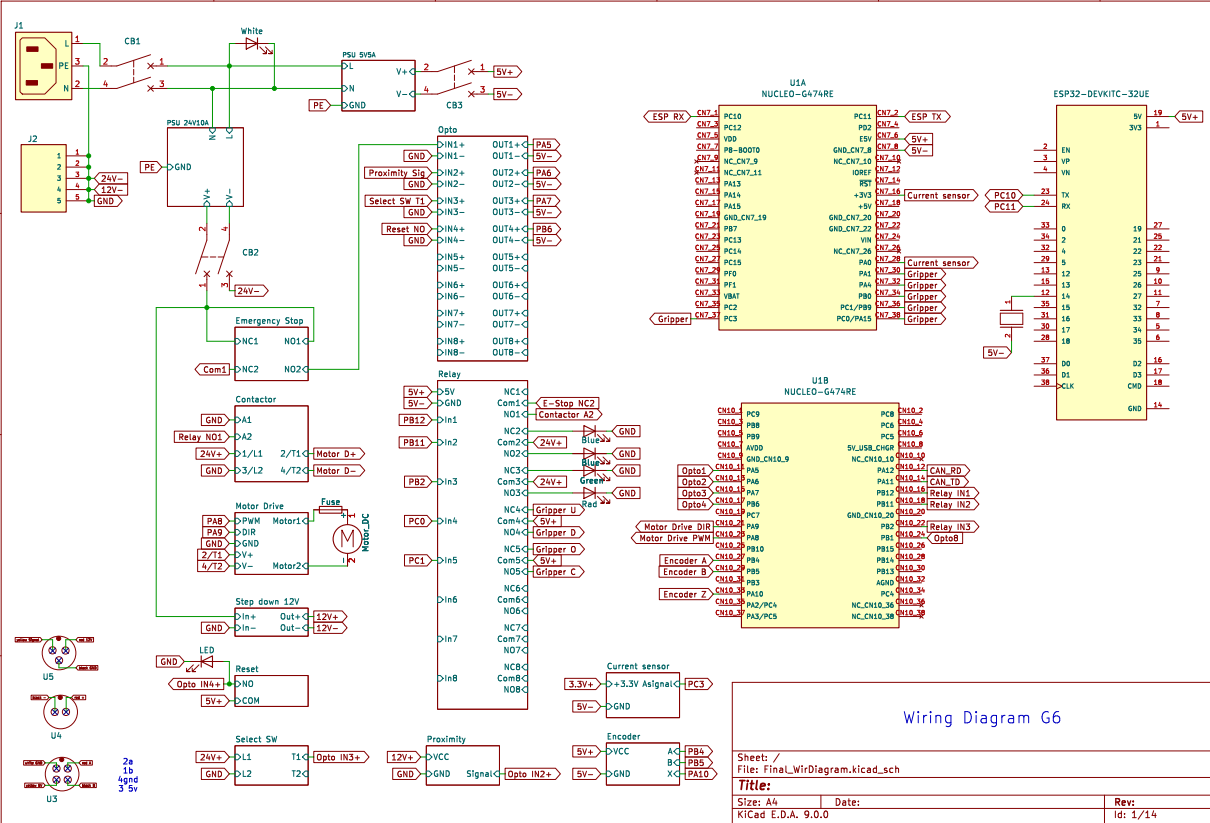
\includegraphics[width=0.95\textwidth]{images/electrical_schematic.png}
  \caption{Electrical Schematic ของตู้ควบคุมทั้งระบบ ออกแบบด้วย KiCad 9.0.0}
  \label{fig:schematic}
\end{figure}

\subsubsection{การออกแบบ PCB (PCB Design)}
\label{subsubsec:pcb_design}
PCB ออกแบบ ด้วย KiCad 9.0.0 เพื่อ รวม STM32G474RE Nucleo Board, ESP32-DEVKITC-32UE 
และ Motor Driver Connector ไว้บน Board เดียวกัน และมี Terminal รองรับการต่อสายไฟจาก 
Optocoupler Module, Relay Module, Encoder Connector  
เพื่อลดจำนวนสายเชื่อมต่อภายในตู้ควบคุมและเพิ่มความเป็นระเบียบ

\begin{figure}[H]
  \centering
  \begin{subfigure}[b]{0.48\textwidth}
    \centering
    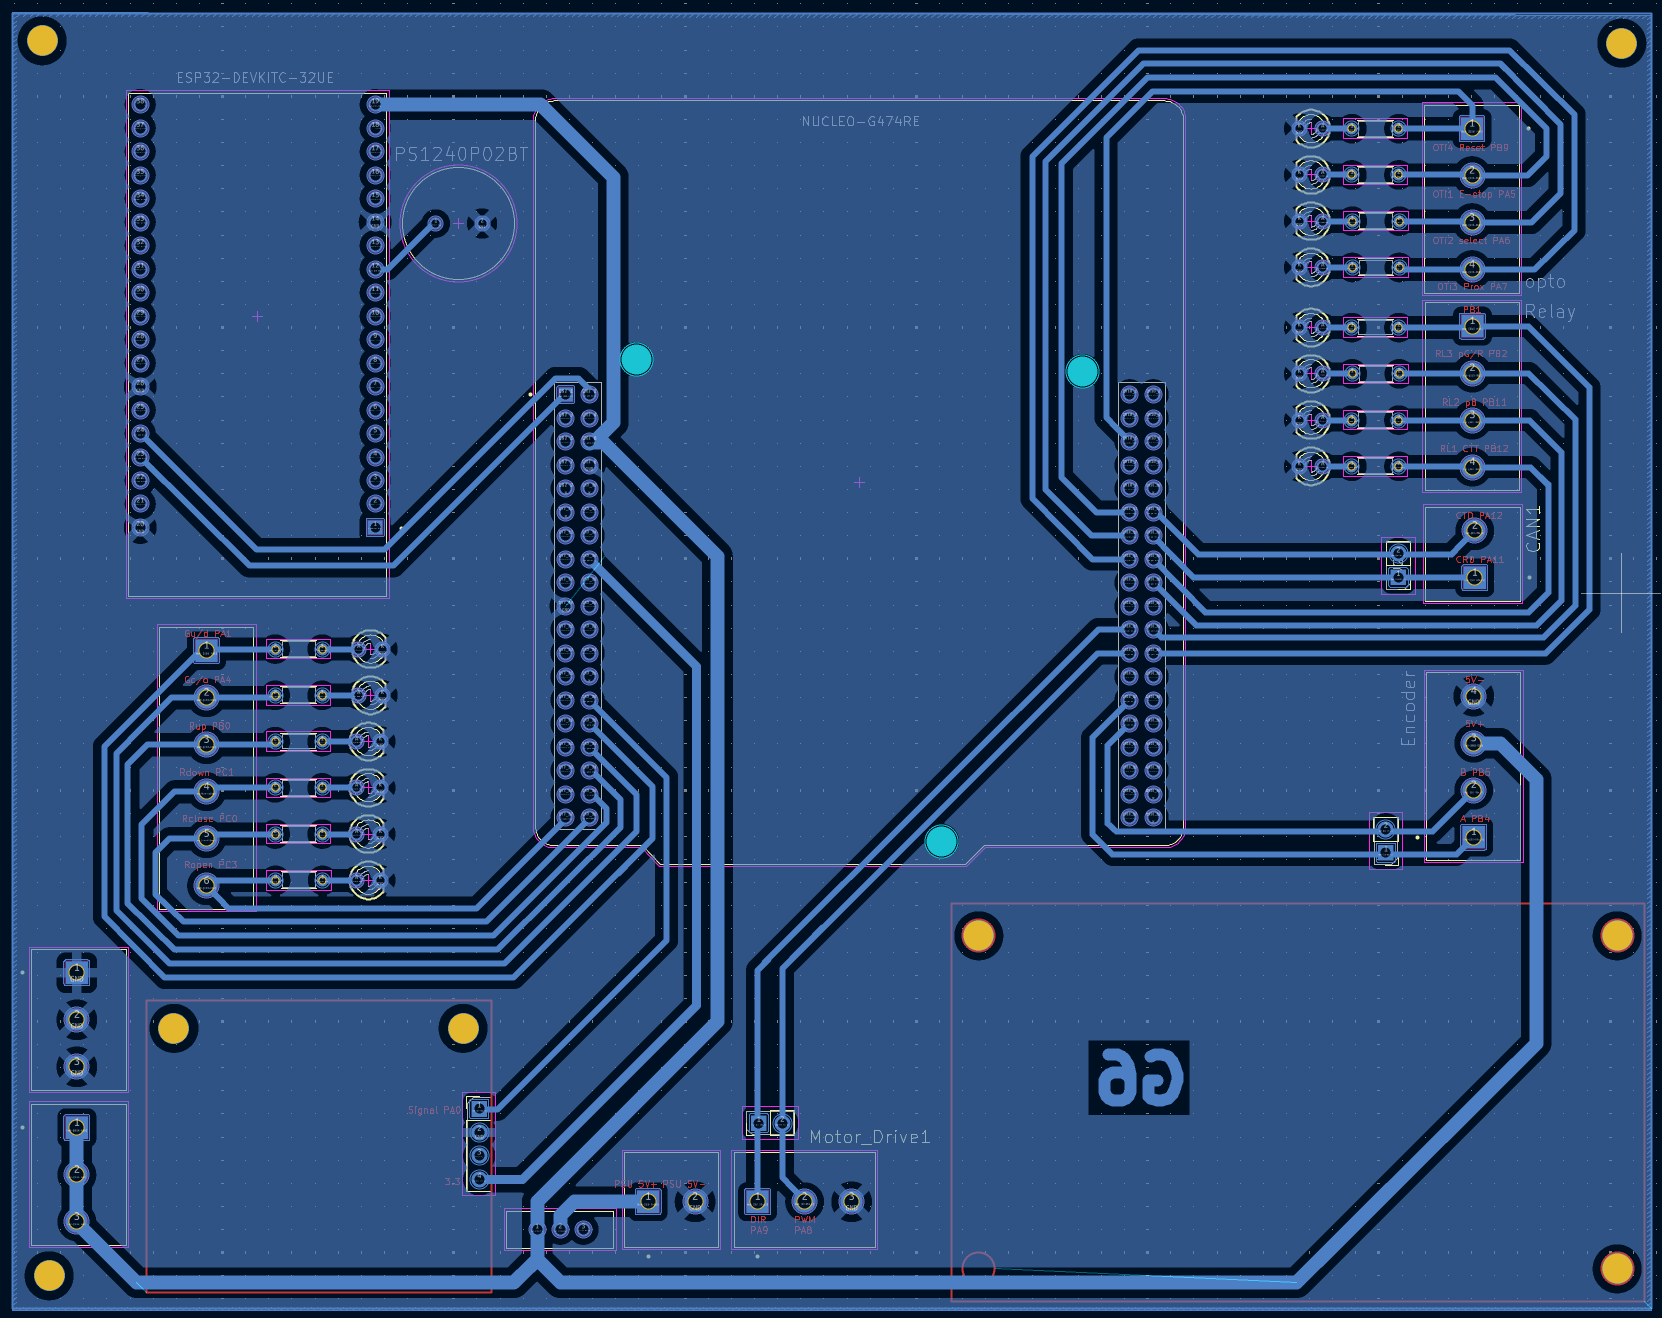
\includegraphics[width=\textwidth]{images/pcb_layout.png}
    \caption{PCB Layout (KiCad PCB Editor)}
    \label{fig:pcb_layout}
  \end{subfigure}
  \hfill
  \begin{subfigure}[b]{0.48\textwidth}
    \centering
    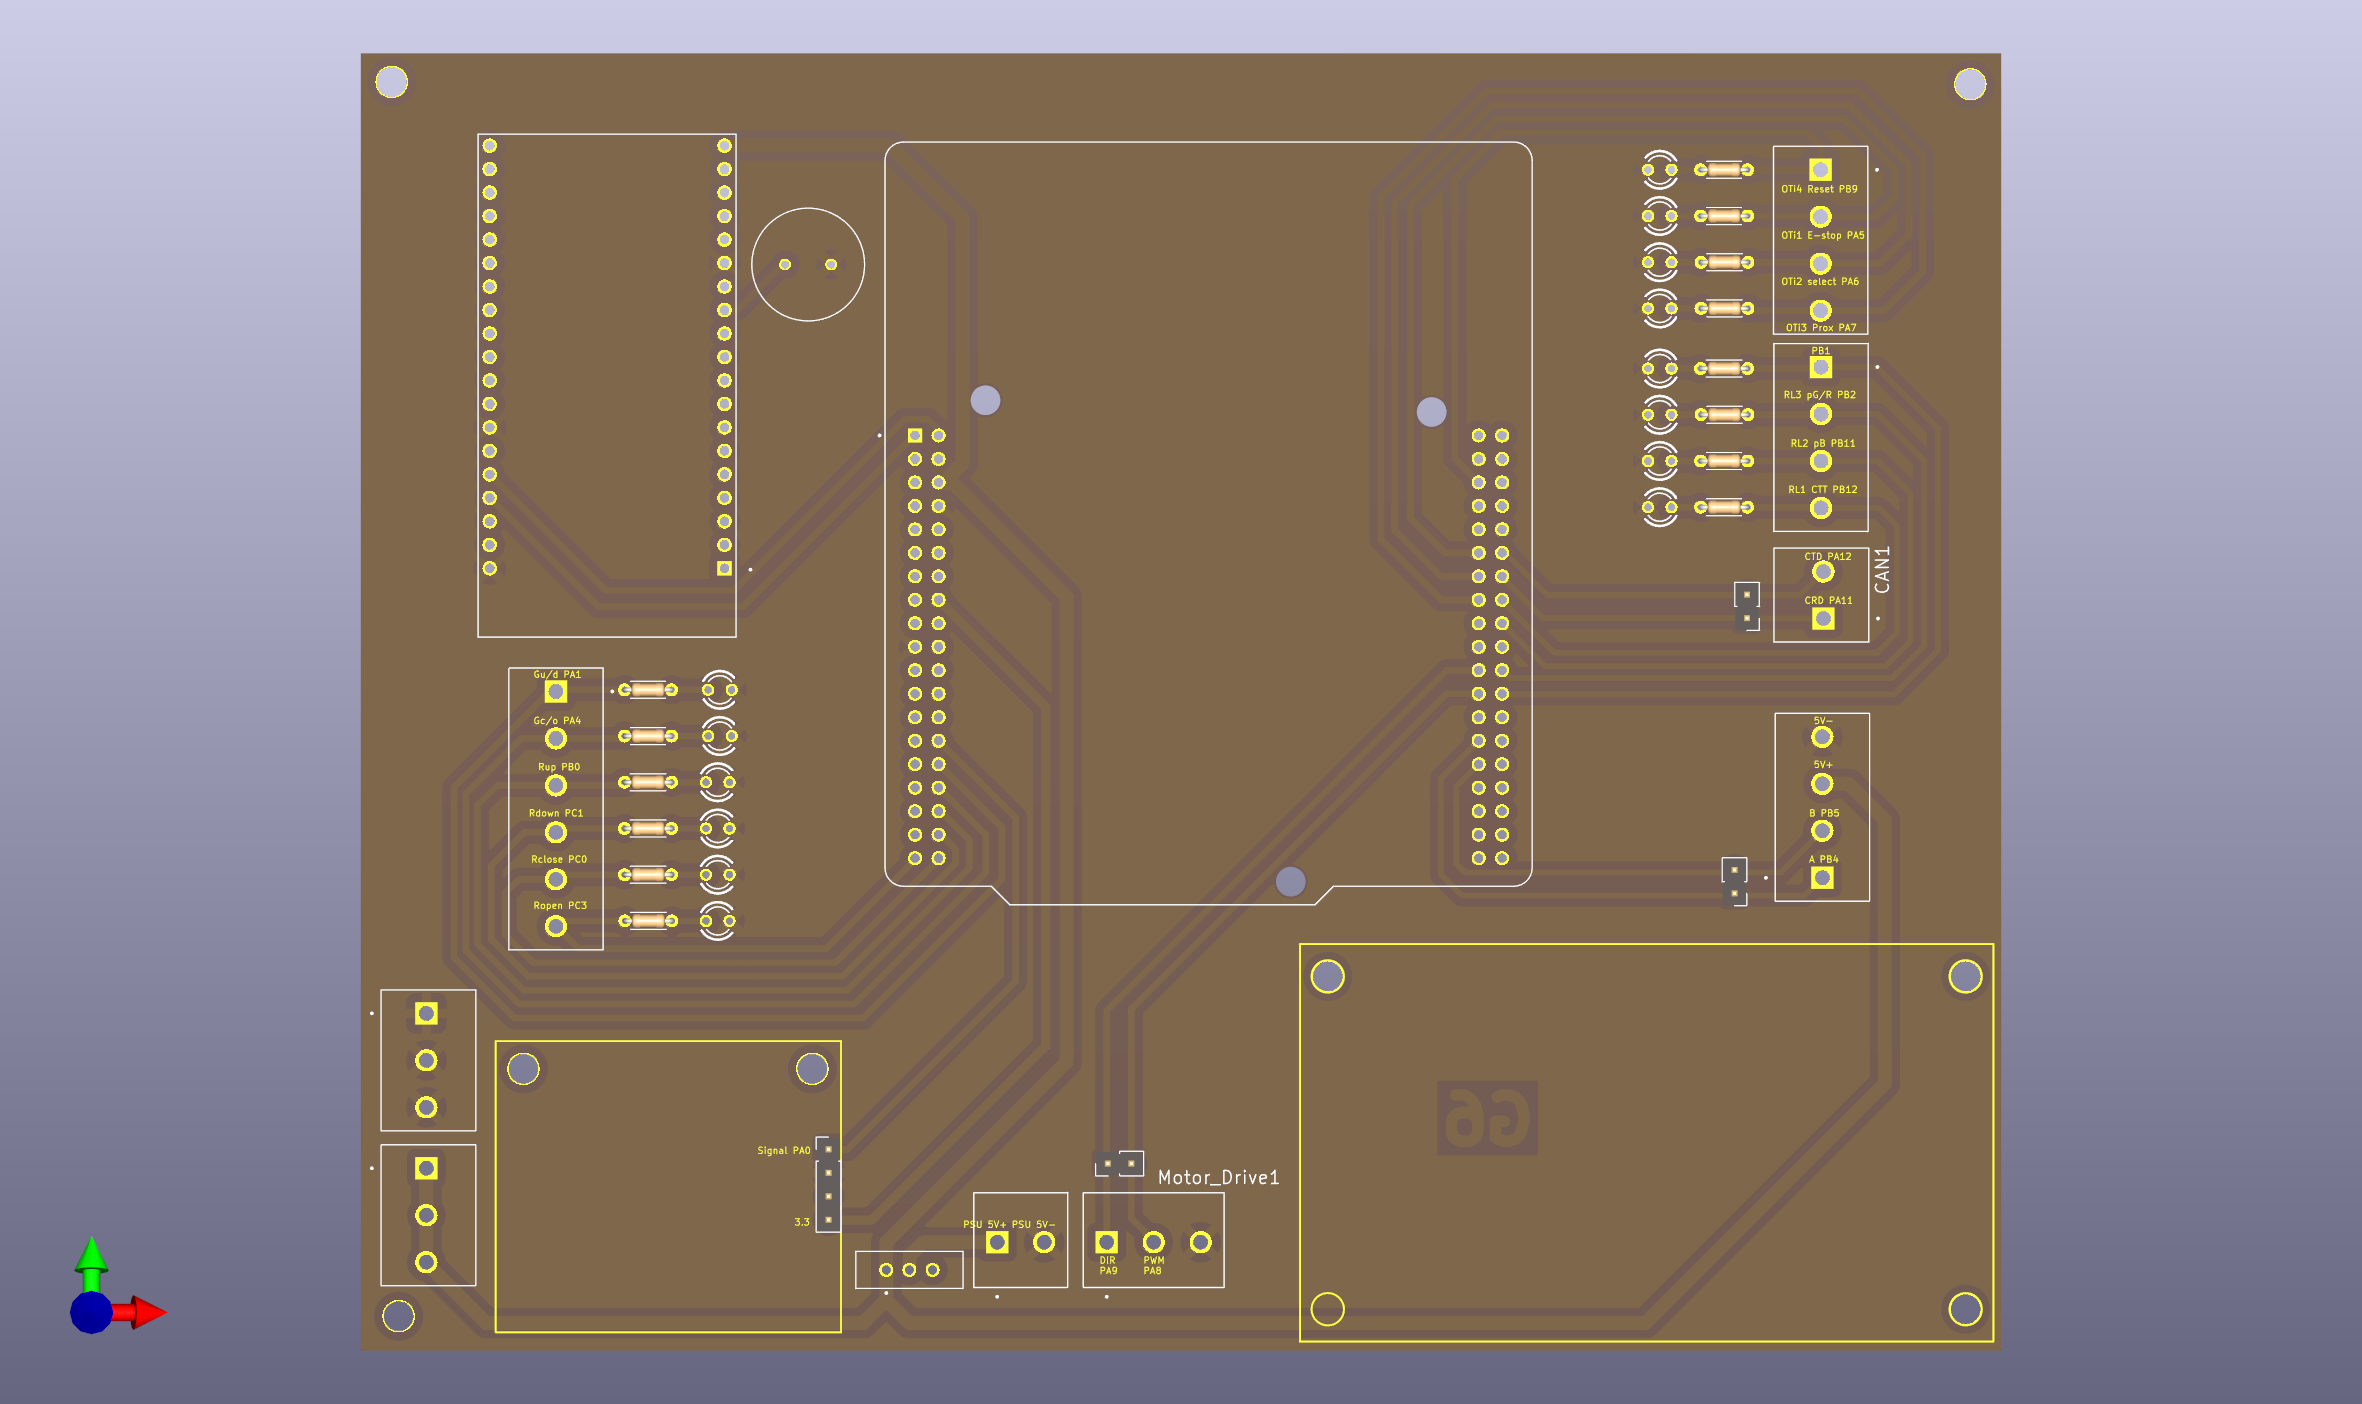
\includegraphics[width=\textwidth]{images/pcb_3d.png}
    \caption{PCB 3D Render}
    \label{fig:pcb_3d}
  \end{subfigure}
  \caption{การออกแบบ PCB สำหรับระบบควบคุม}
  \label{fig:pcb_design}
\end{figure}

% ============================================================
\subsubsection{การออกแบบวงจรป้องกัน (Protection Circuit)}
\label{subsubsec:protection_circuit}
% ============================================================

ระบบมีวงจรป้องกันหลายชั้นตามข้อกำหนด E7 ดังนี้

\textbf{การป้องกัน Overcurrent:}
Circuit Breaker CB1 ทำหน้าที่ป้องกันกระแสเกินพิกัด
ในวงจร AC Input และ CB2 ป้องกันวงจร 24\,V
นอกจากนี้ Cytron MD10C มีวงจรป้องกัน Overcurrent ในตัว
และ Firmware ของ STM32 ตรวจสอบกระแสจาก Current Sensor
ทุก Control Cycle หากเกิน Threshold จะสั่งตัด PWM ทันที

\textbf{การป้องกัน Surge และ Noise:}
Optocoupler Module แยก Ground ระหว่าง High Power Side
และ Logic Side ป้องกัน Surge จากมอเตอร์ไม่ให้ทำลาย STM32
Fuse ต่ออนุกรมในวงจร Motor Driver
เพื่อป้องกันความเสียหายเมื่อเกิด Short Circuit

\textbf{Emergency Stop Hardware Interlock:}
E-Stop ทำงานในระดับ Hardware โดยตรง
ไม่ผ่าน Firmware ทำให้ไม่สามารถ Override ได้แม้ Software ค้าง
NC Contact ของปุ่ม E-Stop ต่ออยู่ใน Series กับ Coil ของ Contactor
เมื่อกด E-Stop หรือสายหลุด Contactor จะ De-energize ทันที
(Fail-Safe Design)

% ============================================================
\subsubsection{การออกแบบวงจร Optocoupler และ Relay}
\label{subsubsec:optocoupler_relay_design}
% ============================================================

Optocoupler Module ทำหน้าที่แปลงสัญญาณระหว่าง
High Voltage Side (24\,V) และ Logic Side (3.3\,V/5\,V ของ STM32)
ใน 2 ทิศทาง ดังแสดงในตารางที่~\ref{tab:opto_mapping}

\begin{table}[H]
  \centering
  \caption{Optocoupler Module Channel Mapping}
  \label{tab:opto_mapping}
  \begin{tabular}{cclll}
    \toprule
    Channel & ทิศทาง & สัญญาณ & STM32 Pin & Mode \\
    \midrule
    CH1 & Input  & Emergency Stop      & PA5  & EXTI Interrupt \\
    CH2 & Input  & Proximity Sensor    & PA6  & GPIO Input \\
    CH3 & Input  & Mode Selector SW    & PA7  & GPIO Input \\
    CH4 & Input  & Reset Button        & PB6  & GPIO Input \\
    CH5 & Output & Relay IN1 (Motor)   & PB12 & GPIO Output \\
    CH6 & Output & Relay IN2 (Mode Lamp) & PB11 & GPIO Output \\
    CH7 & Output & Relay IN3 (Status Lamp) & PB2 & GPIO Output \\
    CH8 & Output & ยังไม่กำหนด        & PB1  & GPIO Output \\
    \bottomrule
  \end{tabular}
\end{table}

Relay Module รับคำสั่งจาก STM32 ผ่าน Optocoupler
และควบคุมอุปกรณ์กำลังสูงดังแสดงในตารางที่~\ref{tab:relay_mapping}

\begin{table}[H]
  \centering
  \caption{Relay Module Channel Mapping}
  \label{tab:relay_mapping}
  \begin{tabular}{cclll}
    \toprule
    Relay & STM32 Pin & COM & NO & NC \\
    \midrule
    IN1 & PB12 & 24\,V (E-Stop NC2) & Contactor A1       & --                  \\
    IN2 & PB11 & 24\,V PSU          & Pilot Blue Joystick & Pilot Blue Base     \\
    IN3 & PB2  & 24\,V PSU          & Pilot Red Emergency & Pilot Green Ready   \\
    IN4 & PC0  & 5\,V PSU           & Gripper Down (High) & Gripper Up (Low)    \\
    IN5 & PC1  & 5\,V PSU           & Gripper Close (High)& Gripper Open (Low)  \\
    \bottomrule
  \end{tabular}
\end{table}

% ============================================================
\subsubsection{STM32 Pin Assignment}
\label{subsubsec:stm32_pin_assignment}
% ============================================================

ตารางที่~\ref{tab:pin_assignment} สรุป Pin Assignment ทั้งหมด
ของ STM32G474RE แบ่งตาม Subsystem

\begin{table}[H]
  \centering
  \caption{STM32G474RE Pin Assignment ของระบบ}
  \label{tab:pin_assignment}
  \begin{tabular}{lllll}
    \toprule
    Pin & Function & Mode & เชื่อมต่อกับ \\
    \midrule
    \multicolumn{4}{l}{\textit{Motor Control}} \\
    PA8 & PWM Output & TIM1 CH1         & Motor Driver PWM \\
    PA9 & DIR Output & GPIO Push-Pull    & Motor Driver DIR \\
    \midrule
    \multicolumn{4}{l}{\textit{Encoder}} \\
    PB4 & Encoder A  & TIM3 CH1 (QEI)   & AMT-103 CH A \\
    PB5 & Encoder B  & TIM3 CH2 (QEI)   & AMT-103 CH B \\
    PA10& Encoder Z  & TIM3 CH3         & AMT-103 Index \\
    \midrule
    \multicolumn{4}{l}{\textit{Communication}} \\
    PC10& UART TX    & USART3 TX        & ESP32 RX (Joystick) \\
    PC11& UART RX    & USART3 RX        & ESP32 TX (Joystick) \\
    PA11& CAN RD     & CAN1\_RD         & CAN Bus \\
    PA12& CAN TD     & CAN1\_TD         & CAN Bus \\
    \midrule
    \multicolumn{4}{l}{\textit{Safety Input (via Optocoupler)}} \\
    PA5 & E-Stop     & EXTI Interrupt   & Opto CH1 \\
    PA6 & Proximity  & GPIO Input       & Opto CH2 \\
    PA7 & Mode SW    & GPIO Input       & Opto CH3 \\
    PB6 & Reset      & GPIO Input       & Opto CH4 \\
    \midrule
    \multicolumn{4}{l}{\textit{Relay Output (via Optocoupler)}} \\
    PB12& Relay IN1  & GPIO Output      & Motor Power Control \\
    PB11& Relay IN2  & GPIO Output      & Mode Pilot Lamp \\
    PB2 & Relay IN3  & GPIO Output      & Status Pilot Lamp \\
    \midrule
    \multicolumn{4}{l}{\textit{Gripper และ Reed Switch}} \\
    PC0 & Gripper UD & GPIO Output      & Relay IN4 (Up/Down) \\
    PC1 & Gripper CO & GPIO Output      & Relay IN5 (Close/Open) \\
    PB0 & Reed Up    & GPIO Output      & Reed SW Up \\
    PA4 & Reed Down  & GPIO Output      & Reed SW Down \\
    PA1 & Reed Close & GPIO Output      & Reed SW Close \\
    PA0 & Reed Open  & GPIO Output      & Reed SW Open \\
    \bottomrule
  \end{tabular}
\end{table}

% [ใส่รูปถ่ายตู้ควบคุมที่เดินสายแล้ว]
\begin{figure}[H]
  \centering
  % [ใส่ภาพถ่ายการเดินสายจริงในตู้ควบคุม]
  \caption{ผลการเดินสายภายในตู้ควบคุมไฟฟ้า}
  \label{fig:cabinet_wiring}
\end{figure}

% ============================================================
\subsubsection{การออกแบบระบบ Joystick}
\label{subsubsec:joystick_system_design}
% ============================================================

ระบบ Joystick ใช้ ESP32-DEVKITC-32UE เป็น Wireless Receiver
รับสัญญาณจาก Joystick ผ่าน Bluetooth แล้วส่งต่อไปยัง STM32
ผ่าน USART3 ที่ Baud Rate 115200\,bps 8N1
ตาม Pin PC10 (TX) และ PC11 (RX)

โปรโตคอลการสื่อสารระหว่าง ESP32 และ STM32
ใช้ Data Packet ที่มีโครงสร้างคงที่
STM32 ถอดรหัส Packet และตรวจสอบ Checksum
ก่อนส่งคำสั่งไปยัง Command Parser ใน Firmware

การ Map ปุ่ม Joystick กับคำสั่งระบบแสดงในตารางที่~\ref{tab:joystick_map}

\begin{table}[H]
  \centering
  \caption{การ Map ปุ่ม Joystick กับคำสั่งระบบ}
  \label{tab:joystick_map}
  \begin{tabular}{lll}
    \toprule
    ปุ่ม Joystick & คำสั่งระบบ & หมายเหตุ \\
    \midrule
    Analog Stick (หมุนซ้าย)  & หมุนแขนซ้าย (Fine/Point) & โหมด Manual เท่านั้น \\
    Analog Stick (หมุนขวา)  & หมุนแขนขวา (Fine/Point) & โหมด Manual เท่านั้น \\
    Button: Home            & Go to Home Position      & ทุกโหมด \\
    Button: Start           & Start Auto Sequence      & โหมด Auto เท่านั้น \\
    Button: E-Stop          & Emergency Stop           & ทุกโหมด \\
    Button: Pick            & Gripper Pick Up          & โหมด Manual เท่านั้น \\
    Button: Place           & Gripper Place Down       & โหมด Manual เท่านั้น \\
    \bottomrule
  \end{tabular}
\end{table}

การสลับโหมดระหว่าง Manual (Joystick) และ Auto (Base System)
ทำผ่าน Mode Selector Switch บนตู้ควบคุม
ซึ่งส่งสัญญาณผ่าน Opto CH3 ไปยัง STM32 PA7
เมื่ออยู่ในโหมด Auto Firmware จะ Block คำสั่งจาก Joystick ทั้งหมด
ยกเว้นคำสั่ง Emergency Stop ซึ่งทำงานได้ทุกโหมดตามข้อกำหนด J1

% ============================================================
% FILE: sections/02_design_control.tex
% PURPOSE: Control Design Section — System Modeling, System ID,
%          PID Design (Loop Shaping), S-Curve, Simulation
% Compiler: XeLaTeX
%
% รูปภาพที่ต้องเตรียม (ใส่ในโฟลเดอร์ images/):
%   motor_circuit.png        -- วงจรสมมูล Armature (วาดใน draw.io)
%   simulink_motor_model.png -- Block diagram จาก Params_Estimate.slx
%   locked_rotor_scope.png   -- Oscilloscope waveform จาก Locked Rotor Test
%   chirp_raw_filtered.png   -- Plot raw vs filtered (จาก preprocess code)
%   cross_validation.png     -- Measured vs Simulated (จาก validate_parameters.m)
%   cross_val_bar.png        -- Bar chart Fit Score (จาก validate_parameters.m)
%   bode_plant.png           -- Bode plot ของ plant (จาก plant_analysis.m)
%   bode_openloop.png        -- Open-loop Bode หลัง design (จาก loop_shaping_design.m)
%   simulink_cascade.png     -- Block diagram cascade PID (screenshot Simulink)
%   scurve_360.png           -- S-curve profile 360° (จาก compute_scurve_v2.m)
%   sim_result.png           -- Simulation result 6 subplots (จาก simulate_cascade_pid_v3.m)
%   sim_current.png          -- Motor current + clamp zone
% ============================================================

% ============================================================
\subsection{การออกแบบระบบควบคุม (Control Design)}
\label{subsec:control_design}
% ============================================================

% ------------------------------------------------------------
\subsubsection{การสร้างแบบจำลองระบบ (System Modeling)}
\label{subsubsec:system_modeling}
% ------------------------------------------------------------

\paragraph{แบบจำลองมอเตอร์กระแสตรง}

ระบบขับเคลื่อนประกอบด้วยมอเตอร์กระแสตรงแบบ Brushed DC Motor
ที่ต่อกับชุดทดรอบแบบ 2 ชั้น ได้แก่ Planetary Gearbox และ Belt Drive
จากนั้นส่งกำลังไปยัง Arm ของหุ่นยนต์ การสร้างแบบจำลองแบ่งออกเป็น
2 ส่วน คือ วงจรไฟฟ้า (Electrical Subsystem) และระบบกล (Mechanical Subsystem)

\paragraph{วงจรไฟฟ้า (Electrical Subsystem)}

วงจรสมมูลของ Armature มอเตอร์กระแสตรงประกอบด้วย
ความต้านทาน $R_a$ ความเหนี่ยวนำ $L_a$ และแรงดันย้อนกลับ (Back-EMF) $e_b$
ดังแสดงใน\cref{fig:motor_circuit} โดยประยุกต์ใช้ Kirchhoff's Voltage Law (KVL)
รอบวงจร Armature ได้สมการ

\begin{equation}
  v_{in}(t) = R_a\, i_a(t) + L_a\, \frac{di_a(t)}{dt} + e_b(t)
  \label{eq:kvl}
\end{equation}

โดยที่ $v_{in}$ คือแรงดันไฟฟ้าอินพุต (V), $i_a$ คือกระแส Armature (A),
$R_a$ คือความต้านทาน Armature ($\Omega$), $L_a$ คือความเหนี่ยวนำ Armature (H)
และ $e_b$ คือแรงดันย้อนกลับ (V)

\begin{figure}[H]
  \centering
  \includegraphics[width=0.65\textwidth]{images/motor_circuit.png}
  \caption{วงจรสมมูลของ Armature มอเตอร์กระแสตรง}
  \label{fig:motor_circuit}
\end{figure}

แรงดันย้อนกลับมีความสัมพันธ์กับความเร็วเชิงมุมของมอเตอร์ ($\omega_m$) ดังนี้

\begin{equation}
  e_b(t) = K_b\, \omega_m(t)
  \label{eq:bemf}
\end{equation}

โดยที่ $K_b$ คือค่าคงที่ Back-EMF (V$\cdot$s/rad)

\paragraph{ระบบกล (Mechanical Subsystem)}

แรงบิดที่มอเตอร์ผลิตได้สัมพันธ์กับกระแส Armature ดังนี้

\begin{equation}
  \tau_m(t) = K_t\, i_a(t)
  \label{eq:torque_motor}
\end{equation}

โดยที่ $K_t$ คือค่าคงที่แรงบิด (N$\cdot$m/A)

\paragraph{ชุดทดรอบ 2 ชั้น}

ระบบใช้ชุดทดรอบแบบ 2 ชั้น ได้แก่ Planetary Gearbox อัตราทดรอบ
$N_g = 24$ และ Belt Drive ที่มี Driver Pulley 24 teeth และ Driven Pulley 70 teeth
ให้อัตราทดรอบ $N_b = 70/24 = 2.917$ อัตราทดรอบรวมคือ

\begin{equation}
  N_{total} = N_g \times N_b = 24 \times \frac{70}{24} = 70
  \label{eq:gear_ratio}
\end{equation}

ความสัมพันธ์ระหว่างความเร็วเชิงมุมและแรงบิดที่ด้าน Output shaft
($\omega_{arm}$, $\tau_{out}$) กับด้าน Motor ($\omega_m$, $\tau_m$) คือ

\begin{equation}
  \omega_{arm}(t) = \frac{\omega_m(t)}{N_{total}}
  \label{eq:omega_arm}
\end{equation}

\begin{equation}
  \tau_{out}(t) = \eta\, N_{total}\, \tau_m(t)
  \label{eq:tau_out}
\end{equation}

โดยที่ $\eta$ คือประสิทธิภาพรวมของชุดทดรอบ

นำ \cref{eq:torque_motor} และ \cref{eq:tau_out} ไปใช้กับ
Newton's Second Law ที่ Output shaft

\begin{equation}
  J\, \frac{d\omega_{arm}(t)}{dt} = \tau_{out}(t) - b\, \omega_{arm}(t)
  \label{eq:newton}
\end{equation}

\begin{equation}
  J\, \frac{d\omega_{arm}(t)}{dt} = \eta\, N_{total}\, K_t\, i_a(t) - b\, \omega_{arm}(t)
  \label{eq:newton_expand}
\end{equation}

โดยที่ $J$ คือโมเมนต์ความเฉื่อยรวมของ Arm, Gripper และ Connection Rod
(kg$\cdot$m$^2$) และ $b$ คือสัมประสิทธิ์การหน่วงแบบ Viscous (N$\cdot$m$\cdot$s/rad)

\paragraph{Block Diagram ของระบบ}

Block Diagram ของแบบจำลองระบบมอเตอร์ที่สร้างใน Simulink
แสดงดัง\cref{fig:motor_block} ซึ่งประกอบด้วย Electrical Loop
ที่ป้อนกลับด้วย Back-EMF และ Mechanical Loop
ที่ป้อนกลับด้วย Viscous Damping

\begin{figure}[H]
  \centering
  \includegraphics[width=0.92\textwidth]{images/simulink_motor_model.png}
  \caption{Block Diagram ของระบบมอเตอร์กระแสตรงพร้อมชุดทดรอบใน Simulink}
  \label{fig:motor_block}
\end{figure}

\paragraph{Transfer Function}

แปลง \cref{eq:kvl,eq:bemf,eq:newton_expand} เป็น Laplace domain
โดยสมมติเงื่อนไขเริ่มต้นเป็นศูนย์

\begin{align}
  V_{in}(s) &= (R_a + L_a s)\, I_a(s) + K_b\, N_{total}\, \Omega_{arm}(s)
  \label{eq:lap_elec} \\
  (Js + b)\, \Omega_{arm}(s) &= \eta\, N_{total}\, K_t\, I_a(s)
  \label{eq:lap_mech}
\end{align}

จาก \cref{eq:lap_mech} แทน $I_a(s)$ ลงใน \cref{eq:lap_elec}
แล้วจัดรูปได้ Velocity Transfer Function ดังนี้

\begin{equation}
  G_{vel}(s) = \frac{\Omega_{arm}(s)}{V_{in}(s)}
             = \frac{\eta K_t N_{total} / (L_a J)}
                    {s^2 + \left(\dfrac{R_a}{L_a} + \dfrac{b}{J}\right)s
                         + \dfrac{R_a b + K_b K_t N_{total}^2}{L_a J}}
  \label{eq:Gvel}
\end{equation}

สำหรับ Position Transfer Function เพิ่ม Integrator เนื่องจาก
$\Theta_{arm}(s) = \Omega_{arm}(s)/s$

\begin{equation}
  G_{pos}(s) = \frac{\Theta_{arm}(s)}{V_{in}(s)}
             = \frac{\eta K_t N_{total} / (L_a J)}
                    {s\left[s^2 + \left(\dfrac{R_a}{L_a} + \dfrac{b}{J}\right)s
                         + \dfrac{R_a b + K_b K_t N_{total}^2}{L_a J}\right]}
  \label{eq:Gpos}
\end{equation}

แทนค่าตัวเลขจาก System Identification

\begin{align}
  K_{num} &= \frac{\eta K_t N_{total}}{L_a J}
           = \frac{0.836 \times 0.04065 \times 70}{0.001448 \times 0.728}
           = \frac{2.376}{0.001054} = 2254 \notag \\
  a_1     &= \frac{R_a}{L_a} + \frac{b}{J}
           = \frac{1.453}{0.001448} + \frac{0.193}{0.728}
           = 1003.5 + 0.265 = 1003.8 \notag \\
  a_0     &= \frac{R_a b + K_b K_t N_{total}^2}{L_a J} \notag \\
           &= \frac{(1.453)(0.193) + (0.04165)(0.04065)(70)^2}{(0.001448)(0.728)} \notag \\
           &= \frac{0.280 + 8.297}{0.001054} = 8136 \notag
\end{align}

ดังนั้น Transfer Function เชิงตัวเลขคือ

\begin{equation}
  G_{vel}(s) = \frac{2254}{s^2 + 1003.8\,s + 8136}
  \label{eq:Gvel_num}
\end{equation}

\begin{equation}
  G_{pos}(s) = \frac{2254}{s\left(s^2 + 1003.8\,s + 8136\right)}
  \label{eq:Gpos_num}
\end{equation}

% ------------------------------------------------------------
\subsubsection{การทำ System Identification}
\label{subsubsec:system_identification}
% ------------------------------------------------------------

\paragraph{พารามิเตอร์ที่วัดโดยตรง: Locked Rotor Test}

ค่า $R_a$ และ $L_a$ วัดด้วย Locked Rotor Test โดยจ่ายแรงดัน Step
ผ่าน Shunt Resistor $R_{sh} = 0.1\,\Omega$ แล้ววัดแรงดันตกคร่อม Shunt
ด้วย Oscilloscope ดังแสดงใน\cref{fig:locked_rotor_scope}
เพื่อหาค่า $V_{max}$ และค่าคงเวลา $\tau$ แล้วคำนวณด้วยสูตร

\paragraph{การเลือกค่า $R_{sh}$}

การเลือกค่า $R_{sh} = 0.1\,\Omega$ มาจากเงื่อนไข 2 ข้อดังนี้

\textbf{เงื่อนไขที่ 1: ไม่รบกวนวงจร}
ค่า $R_{sh}$ ต้องมีขนาดเล็กเมื่อเทียบกับ $R_a$ เพื่อไม่ให้กระทบต่อพฤติกรรมของวงจร
โดยกำหนดค่าคงที่ $k = 0.1$ ดังนี้

\begin{equation}
  \frac{R_{sh}}{R_a} < k \implies R_{sh} < 0.1 \times 1.453 = 0.1453\,\Omega
  \label{eq:rsh_condition1}
\end{equation}

\textbf{เงื่อนไขที่ 2: ทนกำลังไฟได้}
ประมาณกระแส Stall จากแรงดันสูงสุดและค่า $R_a$ ที่วัดได้

\begin{equation}
  I_{stall} \approx \frac{V_{in}}{R_a} = \frac{24}{1.453} \approx 16.5\,\text{A}
  \label{eq:i_stall}
\end{equation}

กำลังที่ $R_{sh}$ ต้องทนได้คือ

\begin{equation}
  P_{sh} = I_{stall}^2 \cdot R_{sh} = (16.5)^2 \times 0.1 \approx 27.2\,\text{W}
  \label{eq:p_sh}
\end{equation}

จากทั้งสองเงื่อนไข จึงเลือก $R_{sh} = 0.1\,\Omega$ 
ซึ่งน้อยกว่าขีดจำกัด $0.1453\,\Omega$ และต้องใช้ตัวต้านทานที่ทนกำลังได้อย่างน้อย $30\,\text{W}$

\paragraph{ที่มาของสูตร}

ขณะ Locked Rotor แกนมอเตอร์หยุดนิ่ง ทำให้ $\omega_m = 0$ 
และ Back-EMF หายไป $e_b = K_b\,\omega_m = 0$ วงจรจึงเหลือเพียง

\begin{equation}
  V_{in} = (R_a + R_{sh})\,i(t) + L_a\,\frac{di(t)}{dt}
  \label{eq:locked_rotor_circuit}
\end{equation}

\textbf{การหา $R_a$:}
ที่ Steady State กระแสนิ่ง $\frac{di}{dt} = 0$ และวัด $V_{sh,ss}$ ได้จาก Oscilloscope
ดังนั้น $i_{ss} = V_{sh,ss}/R_{sh}$ แทนกลับได้

\begin{equation}
  R_a = R_{sh}\left(\frac{V_{in}}{V_{sh,ss}} - 1\right)
  \label{eq:Ra_derive}
\end{equation}

\textbf{การหา $L_a$:}
Solution ของวงจร RL คือ $i(t) = i_{ss}(1 - e^{-t/\tau})$ 
โดยที่ $\tau = L_a/(R_a + R_{sh})$ จัดรูปได้

\begin{equation}
  L_a = \tau\,(R_a + R_{sh}) = R_{sh}\left(\tau\,\frac{V_{in}}{V_{sh,ss}}\right)
  \label{eq:La_derive}
\end{equation}

\begin{equation}
  R_a = R_{sh}\left(\frac{V_{in}}{V_{sh}} - 1\right), \qquad
  L_a = R_{sh}\left(\tau\,\frac{V_{in}}{V_{sh}}\right)
  \label{eq:locked_rotor}
\end{equation}

โดยที่ $V_{sh}$ คือแรงดันตกคร่อม Shunt ที่ Steady State

\begin{figure}[H]
  \centering
  \includegraphics[width=0.70\textwidth]{images/locked_rotor_scope.png}
  \caption{Oscilloscope Waveform จาก Locked Rotor Test แสดง $V_{max}$ และ $\tau$}
  \label{fig:locked_rotor_scope}
\end{figure}

\paragraph{การเลือกแรงดันทดสอบ}

ทดสอบที่แรงดัน 3 ระดับ ได้แก่ $V_{in} = 6$, $9$ และ $12$\,V 
เพื่อตรวจสอบความสม่ำเสมอของค่าที่วัดได้ในแต่ละระดับ
ผลสรุปแสดงในตารางที่~\ref{tab:locked_rotor_all}

\begin{table}[H]
  \centering
  \caption{เปรียบเทียบผลการวัด $R_a$ และ $L_a$ จาก Locked Rotor Test ทั้ง 3 แรงดัน}
  \label{tab:locked_rotor_all}
  \begin{tabular}{ccccc}
    \toprule
    $V_{in}$ (V) & $\bar{R}_a$ ($\Omega$) & $\sigma_{R_a}$ ($\Omega$) 
                 & $\bar{L}_a$ (H)        & $\sigma_{L_a}$ (H) \\
    \midrule
    6  & 1.7300 & 0.0374 & 0.001490 & 0.000062 \\
    9  & 1.5398 & 0.0604 & 0.001473 & 0.000095 \\
    12 & 1.4534 & 0.0523 & 0.001448 & 0.000055 \\
    \bottomrule
  \end{tabular}
\end{table}

จากตารางพบว่าค่า $R_a$ มีแนวโน้มลดลงเมื่อแรงดันเพิ่มขึ้น 
ซึ่งเป็นผลจากสองปัจจัยหลัก ได้แก่
\begin{itemize}
  \item \textbf{Contact Resistance:} ที่แรงดันต่ำ กระแสที่ไหลผ่านน้อย
        ทำให้ความต้านทานสัมผัสของ Brush และขั้วต่อมีนัยสำคัญมากขึ้น
        เมื่อแรงดันสูงขึ้น สัดส่วนของ Contact Resistance ต่อ $R_a$ รวมลดลง
  \item \textbf{Signal-to-Noise Ratio:} ที่ $V_{in} = 6$\,V 
        แรงดันตกคร่อม Shunt $V_{sh}$ มีค่าต่ำ ทำให้ Noise 
        มีผลต่อการอ่านค่ามากกว่า ส่งผลให้ค่าที่วัดได้มี Error สูงกว่า
\end{itemize}

จึงเลือกใช้ผลจาก $V_{in} = 12$\,V เป็นค่าอ้างอิง เนื่องจากสองเหตุผล ได้แก่
\begin{enumerate}
  \item ใกล้เคียงกับแรงดันใช้งานจริง $24$\,V มากที่สุดในบรรดาแรงดันที่ทดสอบ
        ทำให้สภาวะของ Brush Contact ใกล้เคียงกับการทำงานจริงมากที่สุด
  \item ไม่ทดสอบที่ $24$\,V เนื่องจากแขนกลหมุนแรงเกินไป อาจก่อให้เกิดอันตรายได้
\end{enumerate}

เลือกใช้ค่าทดสอบที่ $V_{in} = 12$\,V จำนวน 3 ครั้ง เพื่อหาค่าเฉลี่ยของพารามิเตอร์ทางไฟฟ้า โดยผลการวัดที่ละเอียดแสดงใน\cref{tab:locked_rotor} (บทที่ 5)

ค่าเฉลี่ยที่ได้จากการทดสอบ คือ $R_a = 1.453\,\Omega$ และ $L_a = 1.448\,\text{mH}$
ซึ่งจะใช้เป็นค่าอ้างอิงในการสร้างแบบจำลองและออกแบบระบบควบคุมในหัวข้อถัดไป

\paragraph{การเลือกสัญญาณ Excitation}

เลือกใช้ Chirp Signal เป็น Excitation เนื่องจากเป็นสัญญาณ Sine Wave 
ที่ความถี่เพิ่มขึ้นเรื่อย ๆ ตามเวลา (Frequency Sweep) 
ทำให้สามารถ Excite พฤติกรรมของมอเตอร์ได้ครอบคลุมทั้งย่านความถี่ต่ำ 
(Slow Dynamics เช่น Inertia และ Viscous Damping) 
และย่านความถี่สูง (Fast Dynamics เช่น Friction) ภายใน Input เดียว
สัญญาณอื่น เช่น Step หรือ Impulse มีพลังงานกระจุกตัวอยู่ที่ความถี่เดียว
จึงให้ข้อมูล Frequency Content ที่ไม่ครอบคลุมเท่า

\paragraph{การเลือกย่านความถี่ 0.1--2.0\,Hz}

ขอบล่าง $f_{min} = 0.1$\,Hz เลือกเพื่อให้ครอบคลุม Slow Dynamics
ของระบบ โดยเฉพาะ Inertia $J$ ที่มีผลเด่นชัดที่ความถี่ต่ำมาก

ขอบบน $f_{max} = 2.0$\,Hz กำหนดจาก Dynamics หลักของระบบที่อยู่ในย่านความถี่ต่ำ
เนื่องจากระบบมีอัตราทดรวม $N_{total} = 70$ ทำให้ความเร็วเชิงมุมของแขนกล $\omega_{arm}$
ช้ากว่ามอเตอร์ถึง 70 เท่า Dynamics ที่สำคัญของระบบ ได้แก่ Inertia $J$ และ
Viscous Damping $b$ จึงแสดงผลเด่นชัดในย่านความถี่ต่ำ โดยสามารถประมาณ
Mechanical Bandwidth ของระบบได้จาก

\begin{equation}
    f_{mech} = \frac{1}{2\pi}\sqrt{\frac{R_a b + K_b K_t N^2}{L_a J}}
             = \frac{1}{2\pi}\sqrt{8136}
             \approx 14.4\,\text{Hz}
    \label{eq:f_mech}
\end{equation}

ค่า $f_{max} = 2.0$\,Hz คิดเป็นประมาณ 14\% ของ $f_{mech}$ สะท้อนว่า
Dynamics ส่วนใหญ่ของระบบกระจุกตัวอยู่ในย่านความถี่ต่ำกว่า $f_{mech}$ มาก
อันเป็นผลโดยตรงจากอัตราทดรวมที่สูง

นอกจากนี้ยังเลือกทดสอบ 3 กลุ่มความถี่ ได้แก่
0.1--0.5\,Hz, 0.1--1.0\,Hz และ 0.1--2.0\,Hz
เพื่อตรวจสอบว่าค่าพารามิเตอร์ที่ Estimate ได้มีความสม่ำเสมอในแต่ละย่านความถี่
หากผลการ Estimate แตกต่างกันมากระหว่างกลุ่ม แสดงว่าแบบจำลองอาจไม่เพียงพอ
ในการอธิบาย Dynamics ของระบบในย่านนั้น

\paragraph{การ Preprocess ข้อมูล}

ข้อมูลดิบจาก Hardware กรองด้วย Butterworth Low-pass Filter Order 4
ที่ Cutoff Frequency $f_c = 10$\,Hz โดยเลือกจากเงื่อนไข

\begin{equation}
  f_c = 5 \times f_{max} = 5 \times 2.0 = 10\,\text{Hz}
  \label{eq:fc}
\end{equation}

การเลือก $f_c = 5 f_{max}$ มีเหตุผลสองประการ ประการแรกคือสัญญาณ Chirp
ทุกความถี่ในย่าน $0.1$--$2.0$\,Hz ผ่าน Filter ได้เต็มที่โดยไม่ถูกลด Amplitude
เนื่องจาก $f_{max}$ อยู่ห่างจาก $f_c$ ถึง 5 เท่า ซึ่งอยู่ลึกใน Passband
ประการที่สองคือ Noise ความถี่สูงจาก Encoder Quantization และ Electrical
Interference ซึ่งมักอยู่ในย่านสูงกว่า $f_c$ จะถูกลดทอนลงอย่างมีนัยสำคัญ

เลือก Butterworth เนื่องจากมี Maximally Flat Passband กล่าวคือ
Magnitude Response ในย่าน $0$--$f_c$ ราบเรียบที่สุดในบรรดา Filter
ประเภทเดียวกัน ทำให้ไม่บิดเบือน Amplitude ของสัญญาณในย่านที่สนใจ
ซึ่งมีความสำคัญอย่างยิ่งสำหรับ System Identification เพราะหาก Amplitude
ของ $V_{in}$ หรือ $\omega_{arm}$ ถูกบิดเบือน Parameter Estimator
จะได้ค่า Gain ของระบบผิดพลาดไปด้วย

Order 4 ให้ Rolloff ที่ $-80$\,dB/decade ซึ่งคำนวณได้จาก

\begin{equation}
  A = -20 \times 4 \times \log_{10}\!\left(\frac{10\,f_c}{f_c}\right)
    = -20 \times 4 \times 1
    = -80\,\text{dB}
  \label{eq:attenuation}
\end{equation}

หมายความว่าสัญญาณที่ความถี่ $10 f_c = 100$\,Hz จะถูกลดลงเหลือเพียง

\begin{equation}
  10^{-80/20} = 10^{-4} = 0.01\%
\end{equation}

ของ Amplitude เดิม ซึ่งเพียงพอในการกำจัด Noise ออกจากสัญญาณ
โดยที่ Order 4 ยังไม่สูงจนเกิด Numerical Instability ในการคำนวณ

ใช้ \texttt{filtfilt} แทน \texttt{filter} ธรรมดาเพื่อให้ Phase Shift
เป็นศูนย์ตลอดทุกความถี่ โดย \texttt{filtfilt} ทำงานโดย Filter ข้อมูล
ไปข้างหน้า (Forward) แล้วย้อนกลับ (Backward) อีกครั้ง ทำให้ Phase Shift
ของทั้งสองทิศทางหักล้างกันพอดี เหตุที่ต้องการ Phase Shift เป็นศูนย์คือ
หาก $V_{in}$ และ $\omega_{arm}$ มี Phase Shift ต่างกัน ความสัมพันธ์
เชิงเวลาระหว่างสองสัญญาณจะคลาดเคลื่อน ทำให้ Parameter Estimator
ตีความว่าระบบมี Dynamics ที่ช้าหรือเร็วกว่าความเป็นจริง
ส่งผลให้ค่าพารามิเตอร์ที่ได้ โดยเฉพาะ $L_a$ และ $J$ ผิดพลาดได้

\subsubsection{ขั้นตอนการทำ Parameter Estimation}
\label{subsubsec:parameter_estimation}

การประมาณค่าพารามิเตอร์กระทำด้วยวิธี Grey-box Parameter Estimation
โดยใช้ MATLAB Simulink Parameter Estimator ซึ่งสร้าง Simulink Model
ที่มีโครงสร้างตรงกับสมการ~\eqref{eq:kvl} และ~\eqref{eq:newton_expand}
แล้วให้ Toolbox ปรับค่าพารามิเตอร์โดยใช้ Cost Function แบบ
Sum-Absolute Error จนได้ Output $\omega_{arm}$ ที่ใกล้เคียงกับ
ข้อมูลจริงมากที่สุด

พารามิเตอร์ที่ Fix ไว้จากการวัดโดยตรง ได้แก่ $R_a$, $L_a$ และ $N_{total}$
ส่วนพารามิเตอร์ที่ Estimate พร้อมขอบเขตการค้นหาแสดงในตารางที่~\ref{tab:param_bounds}

\begin{table}[h]
\centering
\caption{ขอบเขตของพารามิเตอร์ที่ใช้ใน Parameter Estimation}
\label{tab:param_bounds}
\begin{tabular}{lccc}
\hline
พารามิเตอร์ & สัญลักษณ์ & Min & Max \\
\hline
Back-EMF Constant   & $K_b$  & 0.001 & 0.5 \\
Torque Constant     & $K_t$  & 0.001 & 0.5 \\
Viscous Damping     & $b$    & 0.0001 & 10 \\
Moment of Inertia   & $J$    & 0.01 & 5 \\
Efficiency          & $\eta$ & 0.3 & 1 \\
\hline
\end{tabular}
\end{table}

ขั้นตอนการ Estimate กระทำซ้ำสำหรับแต่ละชุดข้อมูล ได้แก่
chirp 0.5 Hz, chirp 1 Hz และ chirp 2 Hz โดยแต่ละชุดทดสอบ 3 runs
รวมทั้งสิ้น 9 Experiments จากนั้นนำค่าพารามิเตอร์ที่ได้มาเฉลี่ย
และตรวจสอบความสม่ำเสมอระหว่าง runs ก่อนนำไปใช้ใน
Control Design

\textbf{ผลการตรวจสอบความถูกต้องของแบบจำลอง (Model Validation)}

การตรวจสอบความถูกต้องของแบบจำลองกระทำโดยนำแบบจำลองไปจำลองการทำงานเปรียบเทียบกับข้อมูลจริงจาก Hardware ในเงื่อนไขต่าง ๆ (Cross-Validation) เพื่อคำนวณ Fit Score และ NRMSE โดยค่าพารามิเตอร์ที่ใช้ในแบบจำลองได้มาจากการรวบรวมผลการทดสอบจริงที่แสดงในบทที่ 5 (Test Results) และสรุปไว้ในตารางที่~\ref{tab:sysid_params} ซึ่งรายละเอียดการทดสอบเพิ่มเติมแสดงใน\cref{subsec:model_validation_results}
โดยจะนำค่าไปออกแบบตัวควบคุม PID ด้วยวิธี Root Locus ในหัวข้อถัดไป

\begin{table}[H]
  \centering
  \caption{พารามิเตอร์ที่ได้จาก System Identification (สรุปจากบทที่ 5)}
  \label{tab:sysid_params}
  \begin{tabular}{llccc}
    \toprule
    พารามิเตอร์ & สัญลักษณ์ & ค่า & หน่วย & วิธีการ \\
    \midrule
    Armature Resistance    & $R_a$  & 1.4534   & $\Omega$              & Locked Rotor Test \\
    Armature Inductance    & $L_a$  & 0.001448 & H                     & Locked Rotor Test \\
    Back-EMF Constant      & $K_b$  & 0.04165  & V$\cdot$s/rad         & Parameter Estimation \\
    Torque Constant        & $K_t$  & 0.04065  & N$\cdot$m/A           & Parameter Estimation \\
    Viscous Damping        & $b$    & 0.19279  & N$\cdot$m$\cdot$s/rad & Parameter Estimation \\
    Moment of Inertia      & $J$    & 0.72762  & kg$\cdot$m$^2$        & Parameter Estimation \\
    Gear Ratio (Planetary) & $N_g$  & 24       & --                    & Datasheet \\
    Belt Drive Ratio       & $N_b$  & 2.917    & --                    & การออกแบบ \\
    Total Gear Ratio       & $N$    & 70       & --                    & $N_g \times N_b$ \\
    Efficiency             & $\eta$ & 0.836    & --                    & Parameter Estimation \\
    \bottomrule
  \end{tabular}
\end{table}

% ------------------------------------------------------------
\subsubsection{การออกแบบตัวควบคุม PID ด้วย Root Locus}
\label{subsubsec:pid_design}
% ------------------------------------------------------------

\paragraph{โครงสร้างระบบควบคุม}

ระบบควบคุมใช้โครงสร้าง Cascade PID Control
ซึ่งประกอบด้วย 2 Loop ซ้อนกัน ดังแสดงใน\cref{fig:cascade_block}
โดย Velocity Inner Loop ทำหน้าที่ควบคุมความเร็วเชิงมุม $\omega_{arm}$
และ Position Outer Loop ทำหน้าที่ควบคุมตำแหน่ง $\theta_{arm}$
พร้อมด้วย Velocity Feedforward และ Acceleration Feedforward
เพื่อลด Tracking Error

\begin{figure}[H]
  \centering
  \includegraphics[width=0.95\textwidth]{images/simulink_cascade.png}
  \caption{Block Diagram ของ Cascade PID Control พร้อม Feedforward}
  \label{fig:cascade_block}
\end{figure}

\paragraph{ข้อกำหนดการออกแบบ}

\begin{table}[H]
  \centering
  \caption{ข้อกำหนดของระบบควบคุม}
  \label{tab:ctrl_req}
  \begin{tabular}{llcc}
    \toprule
    ข้อกำหนด & สัญลักษณ์ & ค่า & รหัส \\
    \midrule
    Settling Time & $t_s$  & $\leq 0.5$ s & P5 \\
    Overshoot     & $\%OS$ & $\leq 1\%$   & P6 \\
    \bottomrule
  \end{tabular}
\end{table}

\paragraph{การวิเคราะห์ Frequency Response ของ Plant}

ก่อนการออกแบบ Controller จำเป็นต้องวิเคราะห์ Frequency Response 
ของ Plant ก่อน เพื่อทำความเข้าใจพฤติกรรมของระบบในแต่ละย่านความถี่
โดยใช้ Bode Plot ซึ่งประกอบด้วยกราฟ 2 ส่วน ได้แก่

\begin{itemize}
  \item \textbf{Magnitude (dB):} แสดงอัตราส่วนขนาดระหว่าง Output และ Input 
        ที่แต่ละความถี่ เช่น $-20$\,dB หมายความว่า Output มีขนาดเล็กกว่า 
        Input อยู่ 10 เท่า ค่า 0\,dB หมายความว่า Output มีขนาดเท่ากับ Input พอดี
  \item \textbf{Phase (deg):} แสดงความล่าช้าของ Output เทียบกับ Input 
        ที่แต่ละความถี่ เช่น $-90°$ หมายความว่า Output ตามหลัง Input อยู่ 
        $\frac{1}{4}$ คาบของสัญญาณนั้น
\end{itemize}

\textbf{Velocity Plant และ Position Plant}

ระบบนี้ใช้ Plant 2 แบบขึ้นอยู่กับ Output ที่สนใจ ได้แก่

\begin{itemize}
  \item $G_{vel}(s)$: Input คือ $V_{in}$ และ Output คือ $\omega_{arm}$ 
        ใช้สำหรับออกแบบ Velocity Inner Loop
  \item $G_{pos}(s)$: Input คือ $V_{in}$ และ Output คือ $\theta_{arm}$ 
        ใช้สำหรับออกแบบ Position Outer Loop
\end{itemize}

ความสัมพันธ์ระหว่างทั้งสองคือ

\begin{equation}
  G_{pos}(s) = \frac{G_{vel}(s)}{s}
  \label{eq:gpos_gvel}
\end{equation}

การหาร $s$ เท่ากับการเพิ่ม Integrator หนึ่งตัว ส่งผลให้ Phase ของ 
$G_{pos}(s)$ ต่ำกว่า $G_{vel}(s)$ อยู่ $90°$ ตลอดทุกความถี่
ดังที่เห็นในรูปที่~\ref{fig:bode_plant} ว่า Phase ของ $G_{pos}(s)$ 
เริ่มต้นที่ $-90°$ แทนที่จะเริ่มที่ $0°$ เหมือน $G_{vel}(s)$

\textbf{การเลือก Damping Ratio $\zeta = 0.85$}

Damping Ratio $\zeta$ กำหนดจาก Overshoot Requirement ที่ระบุไว้ใน P6 
ว่า OS $\leq 1\%$ โดย Solve หาค่า $\zeta$ ขั้นต่ำที่ทำให้เงื่อนไขนี้สำเร็จ
จากสมการ Overshoot ของระบบ Second-Order

\begin{equation}
  \%OS = e^{-\pi\zeta/\sqrt{1-\zeta^2}} \times 100 \leq 1
  \label{eq:os_requirement}
\end{equation}

จัดรูปสมการโดยนำ Log ทั้งสองข้าง

\begin{equation}
  \frac{\pi\zeta}{\sqrt{1-\zeta^2}} \geq -\ln\!\left(\frac{1}{100}\right) 
  = \ln(100) = 4.605
  \label{eq:os_log}
\end{equation}

แก้สมการหา $\zeta$ ขั้นต่ำได้

\begin{equation}
  \zeta_{min} = \frac{4.605}{\sqrt{\pi^2 + 4.605^2}} 
              = \frac{4.605}{\sqrt{9.870 + 21.206}} 
              = \frac{4.605}{5.575} 
              \approx 0.826
  \label{eq:zeta_min}
\end{equation}

จึงเลือก $\zeta = 0.85$ ซึ่งสูงกว่าขีดจำกัด $\zeta_{min} = 0.826$ 
เพื่อให้มี Margin เพียงพอสำหรับความไม่แน่นอนของระบบจริง
และยืนยันได้ว่าได้ Overshoot จริงคือ

\begin{equation}
  \%OS = e^{-\pi(0.85)/\sqrt{1-0.85^2}} \times 100 
       = e^{-\pi(0.85)/0.527} \times 100 
       = 0.43\%
  \label{eq:os_verify}
\end{equation}

ซึ่งต่ำกว่าเกณฑ์ $1\%$ อย่างชัดเจน

\textbf{Phase Margin และความสำคัญต่อเสถียรภาพ}

จุดสำคัญที่ต้องอ่านจาก Bode Plot ก่อนออกแบบ Controller มีสองจุด ได้แก่

\begin{itemize}
  \item \textbf{Gain Crossover Frequency ($\omega_c$):} คือความถี่ที่ 
        Magnitude $= 0$\,dB หมายความว่าที่ความถี่นี้ Output มีขนาดเท่ากับ 
        Input พอดี $\omega_c$ บอกถึงความเร็วในการตอบสนองของระบบ 
        Closed-Loop ยิ่ง $\omega_c$ สูง ระบบยิ่งตอบสนองเร็ว

  \item \textbf{Phase Margin (PM):} คือระยะห่างระหว่าง Phase ที่ $\omega_c$ 
        กับ $-180°$ คำนวณได้จาก
        \begin{equation}
          PM = 180° + \angle G(j\omega_c)
          \label{eq:phase_margin}
        \end{equation}
        ยิ่ง PM สูง ระบบยิ่ง Stable และมี Overshoot น้อย 
        หาก PM ต่ำกว่า $0°$ ระบบจะ Oscillate ไม่หยุด
\end{itemize}

\textbf{ความสำคัญของ Phase Margin ต่อการออกแบบ}

เหตุที่ต้องติดตาม PM อย่างใกล้ชิดเนื่องจากระบบ Closed-Loop
จะไม่เสถียรเมื่อสัญญาณวนรอบ Feedback Loop แล้วกลับมาเสริมตัวเอง
ซึ่งเกิดขึ้นพร้อมกันสองเงื่อนไขคือ Loop Gain $\geq 1$ และ Phase $= -180°$
เพราะ $-180°$ ทำให้ Negative Feedback กลายเป็น Positive Feedback
PM จึงเป็นตัววัดว่าระบบอยู่ห่างจากเงื่อนไขอันตรายนี้เพียงใด

นอกจากเสถียรภาพแล้ว PM ยังสัมพันธ์โดยตรงกับ Overshoot
ของระบบ Closed-Loop ผ่านความสัมพันธ์ประมาณ

\begin{equation}
  PM \approx 100\,\zeta
  \label{eq:pm_zeta}
\end{equation}

โดยที่ $\zeta$ คือ Damping Ratio ของระบบ Closed-Loop
และ Overshoot สัมพันธ์กับ $\zeta$ ด้วยสมการ

\begin{equation}
  \%OS = e^{-\pi\zeta/\sqrt{1-\zeta^2}} \times 100
  \label{eq:overshoot}
\end{equation}

ข้อกำหนด P6 กำหนด Overshoot $\leq 1\%$ ซึ่ง Solve จากสมการ~\eqref{eq:overshoot}
ได้ $\zeta_{min} = 0.826$ และจากสมการ~\eqref{eq:pm_zeta} ได้

\begin{equation}
  PM_{required} \approx 100 \times 0.826 = 82.6°
  \label{eq:pm_required}
\end{equation}

จากรูปที่~\ref{fig:bode_plant} พบว่า $G_{pos}(s)$ มี Phase 
ต่ำกว่า $-135°$ ในย่าน $\omega > 5$\,rad/s หมายความว่า 
PM $< 45°$ ซึ่งน้อยกว่า $PM_{required} = 82.6°$ อย่างมีนัยสำคัญ
จึงจำเป็นต้องออกแบบ PID Controller เพื่อยก Phase ขึ้น

\begin{figure}[H]
  \centering
  \includegraphics[width=0.88\textwidth]{images/bode_plant.png}
  \caption{Bode Plot ของ Velocity Plant $G_{vel}(s)$ และ Position Plant $G_{pos}(s)$}
  \label{fig:bode_plant}
\end{figure}

\paragraph{การออกแบบ Velocity Inner Loop}

\textbf{ทำไมต้องเร็วกว่า Position Loop 5 เท่า}

ระบบ Cascade Control ประกอบด้วย 2 Loop ซ้อนกัน โดย Velocity Inner Loop
ทำหน้าที่ควบคุมความเร็ว และ Position Outer Loop ทำหน้าที่ควบคุมตำแหน่ง
หลักการออกแบบ Cascade Control กำหนดให้ Inner Loop ต้องตอบสนองเร็วกว่า
Outer Loop อย่างน้อย 3--10 เท่า เพื่อให้ Outer Loop มองเห็น Inner Loop
เป็นเสมือน Ideal Follower ที่ตามคำสั่งได้ทันที
หากความเร็วของทั้งสอง Loop ใกล้เคียงกัน Loop ทั้งสองจะ Interact กัน
ทำให้ระบบไม่เสถียร จึงเลือก 5 เท่าเป็นค่ากลางที่ปลอดภัย

\begin{equation}
  \omega_{c,vel} \geq 5\,\omega_{c,pos} = 5 \times 9.41 = 47.1\,\text{rad/s}
  \quad \Rightarrow \quad
  \omega_{c,vel} = 47\,\text{rad/s}
\end{equation}

\textbf{ที่มา of Phase $-82.8°$ ที่ $\omega = 47$\,rad/s}

Transfer Function ของ Velocity Plant คือ

\begin{equation}
  G_{vel}(s) = \frac{2254}{s^2 + 1003.8\,s + 8136}
\end{equation}

แทน $s = j\omega = j47$ เพื่อหา Phase

\begin{equation}
  \begin{split}
    G_{vel}(j47) &= \frac{2254}{(j47)^2 + 1003.8(j47) + 8136} \\
                 &= \frac{2254}{(8136 - 47^2) + j(1003.8 \times 47)} \\
                 &= \frac{2254}{5927 + j47{,}179}
  \end{split}
  \label{eq:gvel_j47}
\end{equation}

Phase ของ $G_{vel}(j47)$ คือ Phase ของตัวส่วน ซึ่งเป็น Complex Number

\begin{equation}
  \angle G_{vel}(j47) = -\arctan\!\left(\frac{47{,}179}{5927}\right)
                      = -\arctan(7.960)
                      = -82.8°
  \label{eq:vel_phase}
\end{equation}

หมายความว่า Plant เปล่าๆ ที่ $\omega_c = 47$\,rad/s มี Phase อยู่ที่ $-82.8°$
ดังนั้น Phase Margin ของ Plant เปล่าๆ คือ $180° - 82.8° = 97.2°$
ซึ่งสูงกว่าเกณฑ์ $70°$ แต่ยังต้องใส่ PID เพื่อปรับ Gain ให้ถูกต้อง
โดยใช้ \texttt{pidtune} ของ MATLAB ออกแบบที่ $\omega_c = 47$\,rad/s
และ $PM = 70°$ ได้ Phase Margin จริง $79.2°$

\paragraph{การออกแบบ Position Outer Loop}

กำหนด $\omega_{c,pos}$ จาก Settling Time Requirement P5 
ที่ระบุว่า $t_s \leq 0.5$\,s โดยใช้ความสัมพันธ์ของระบบ Second-Order

\begin{equation}
  \omega_{c,pos} = \frac{4}{\zeta\, t_s}
                = \frac{4}{0.85 \times 0.5}
                = 9.41\,\text{rad/s}
\end{equation}

ซึ่งยืนยันได้จากรูปที่~\ref{fig:bode_plant} ว่าที่ $\omega = 9.41$\,rad/s
Phase ของ $G_{pos}$ ต่ำกว่า $-135°$ แล้ว จึงต้องออกแบบ
Controller ให้ได้ PM $\geq 80°$ ที่ความถี่นี้

และกำหนด $PM_{pos} \geq 80°$ เพื่อให้ได้ Damping ที่สอดคล้องกับ
$\zeta = 0.85$ ในระบบ Closed-Loop จริง
โดยใช้ความสัมพันธ์ประมาณ $PM \approx 100\zeta = 85°$
แล้วเลือก $80°$ เป็นขีดจำกัดขั้นต่ำเพื่อให้มี Margin

Open-loop Bode Plot หลัง design แสดงดัง\cref{fig:bode_openloop}

\begin{figure}[H]
  \centering
  \includegraphics[width=0.88\textwidth]{images/bode_openloop.png}
  \caption{Open-loop Bode Plot ของ Velocity Loop และ Position Loop หลัง Design
           แสดง Crossover Frequency และ Phase Margin}
  \label{fig:bode_openloop}
\end{figure}

\paragraph{Feedforward Gains}

\textbf{ทำไมต้องมี Feedforward เพิ่มจาก PID}

PID Controller ทำงานแบบ Reactive คือรอให้เกิด Error ก่อนแล้วจึงแก้ไข
ในขณะที่ S-Curve Profile เปลี่ยน Reference ตลอดเวลา
ทำให้ PID มี Tracking Error สะสมตลอดช่วงการเคลื่อนที่
Feedforward แก้ปัญหานี้โดยคำนวณ Voltage ที่ต้องการล่วงหน้า
จาก Reference Velocity และ Acceleration โดยตรง
ทำให้ PID ต้องแก้ไขแค่ส่วนที่เหลือจาก Model Error เท่านั้น

\textbf{ที่มา of สูตร $K_{vff}$}

ที่ Steady State ความเร่งเป็นศูนย์ $\dot{\omega}_{arm} = 0$
สมการกลของระบบที่ Output Shaft คือ

\begin{equation}
  0 = \eta\, N\, K_t\, i_a - b\,\omega_{arm}
  \quad \Rightarrow \quad
  i_a = \frac{b\,\omega_{arm}}{\eta\, N\, K_t}
  \label{eq:ia_ss}
\end{equation}

แทนลงในสมการไฟฟ้าที่ Steady State ($\frac{di_a}{dt} = 0$)

\begin{equation}
  V_{in} = R_a\, i_a + K_b\, N\,\omega_{arm}
         = \frac{R_a\, b}{\eta\, N\, K_t}\,\omega_{arm} + K_b\, N\,\omega_{arm}
  \label{eq:vin_ss}
\end{equation}

ดังนั้น Velocity Feedforward Gain คือ

\begin{equation}
  \begin{split}
    K_{vff} &= \frac{V_{in}}{\omega_{arm}}
             = \frac{R_a\, b}{\eta\, N\, K_t} + K_b\, N \\
            &= \frac{1.453 \times 0.193}{0.04065 \times 0.836 \times 70}
               + 0.04165 \times 70 \\
            &= 0.118 + 2.916 = 3.034\,\text{V/(rad/s)}
  \end{split}
  \label{eq:Kvff}
\end{equation}

\textbf{ที่มา of สูตร $K_{aff}$}

ในช่วงเร่ง $\dot{\omega}_{arm} \neq 0$ สมการกลเพิ่ม Inertia Term

\begin{equation}
  J\,\dot{\omega}_{arm} = \eta\, N\, K_t\, i_a - b\,\omega_{arm}
  \quad \Rightarrow \quad
  i_a = \frac{J\,\dot{\omega}_{arm} + b\,\omega_{arm}}{\eta\, N\, K_t}
  \label{eq:ia_accel}
\end{equation}

ส่วนที่เพิ่มขึ้นเนื่องจาก Acceleration คือ

\begin{equation}
  \Delta V_{in} = R_a \cdot \frac{J\,\dot{\omega}_{arm}}{\eta\, N\, K_t}
  \label{eq:dvin_accel}
\end{equation}

ดังนั้น Acceleration Feedforward Gain คือ

\begin{equation}
  K_{aff} = \frac{\Delta V_{in}}{\dot{\omega}_{arm}}
           = \frac{R_a\, J}{\eta\, N\, K_t}
           = \frac{1.453 \times 0.728}{0.04065 \times 0.836 \times 70}
           = \frac{1.057}{2.376} = 0.445\,\text{V/(rad/s}^2\text{)}
  \label{eq:Kaff}
\end{equation}

\paragraph{Filter Coefficient $N$ และหน่วยของ PID Gains}

\textbf{Filter Coefficient $N$ คืออะไร}

Derivative Term ของ PID ในทางทฤษฎีคือ $K_d \cdot s$ ซึ่งเป็น Pure Differentiator
มีปัญหาคือขยาย Noise ความถี่สูงอย่างไม่จำกัด
ในทางปฏิบัติจึงใส่ Low-pass Filter เข้าไปใน Derivative Term ดังนี้

\begin{equation}
  D(s) = K_d \cdot \frac{N\,s}{s + N}
  \label{eq:derivative_filter}
\end{equation}

โดยที่ $N$ คือ Filter Coefficient ซึ่งกำหนด Cutoff Frequency ของ Filter
ที่ $\omega = N$\,rad/s ยิ่ง $N$ สูง Filter ตัด Noise ได้น้อยลง
แต่ Derivative ทำงานได้แม่นยำขึ้นในย่านความถี่สูง
เลือก $N_{vel} = 100$ สำหรับ Velocity Loop เพราะต้องการ Derivative
ที่ทำงานได้ถึง $\omega = 100$\,rad/s ซึ่งสูงกว่า $\omega_{c,vel} = 47$\,rad/s
และเลือก $N_{pos} = 20$ สำหรับ Position Loop เพราะ $\omega_{c,pos} = 9.41$\,rad/s
ต้องการ Derivative ที่ทำงานได้ถึง $\omega = 20$\,rad/s เท่านั้น

\paragraph{สรุปค่า PID Gains}

\begin{table}[H]
  \centering
  \caption{ค่า PID Gain ของระบบควบคุม}
  \label{tab:pid_gains}
  \begin{tabular}{llccc}
    \toprule
    Loop & Gain & สัญลักษณ์ & ค่า & หน่วย \\
    \midrule
    \multirow{4}{*}{Velocity Inner} & Proportional & $K_{p,vel}$ & 20.036  & V/(rad/s) \\
                                    & Integral     & $K_{i,vel}$ & 376.923 & V/rad \\
                                    & Derivative   & $K_{d,vel}$ & 0.0325  & V$\cdot$s/rad \\
                                    & Filter Coeff & $N_{vel}$   & 100     & -- \\
    \midrule
    \multirow{4}{*}{Position Outer} & Proportional & $K_{p,pos}$ & 9.267  & s$^{-1}$ \\
                                    & Integral     & $K_{i,pos}$ & 10.50  & s$^{-2}$ \\
                                    & Derivative   & $K_{d,pos}$ & 0.08   & s \\
                                    & Filter Coeff & $N_{pos}$   & 20     & -- \\
    \midrule
    \multirow{2}{*}{Feedforward}    & Velocity FF  & $K_{vff}$   & 3.034  & V/(rad/s) \\
                                    & Accel FF     & $K_{aff}$   & 0.445  & V/(rad/s$^2$) \\
    \bottomrule
  \end{tabular}
\end{table}

\paragraph{หมายเหตุเกี่ยวกับค่า PID Gains}

ค่า PID Gains ในตารางที่~\ref{tab:pid_gains} ได้มาจากการออกแบบด้วยวิธี 
Loop Shaping โดยใช้ \texttt{pidtune} ของ MATLAB 
และตรวจสอบสมรรถนะด้วยการ Simulate บน State Space Model 
ที่ Discretize ด้วยวิธี Zero-Order Hold (ZOH) ที่ Sampling Rate 10\,kHz
พารามิเตอร์เหล่านี้จะถูกนำไปใช้ในการประเมินสมรรถนะผ่านการ Simulation โดยผลการวิเคราะห์เปรียบเทียบกับ Requirement แสดงใน\cref{subsec:sim_results_arm}

อย่างไรก็ตาม ค่าเหล่านี้ยังเป็นค่าจากการออกแบบทางทฤษฎีบน Model เท่านั้น
ในการใช้งานจริงบน Hardware อาจจำเป็นต้องปรับ Fine-tune 
เนื่องจากปัจจัยที่ Model ไม่ได้คำนึงถึง เช่น Static Friction (Stiction) 
ของ Bearing และ Belt Drive, Backlash ของ Gearbox, Quantization Error 
ของ Encoder และ Sampling Rate จริงของ STM32 ที่ 40\,Hz

% ------------------------------------------------------------
\subsubsection{Motion Profile แบบ S-Curve}
\label{subsubsec:scurve_motion_profile}
% ------------------------------------------------------------

\paragraph{ขีดจำกัดของการเคลื่อนที่}

ขีดจำกัดของ Motion Profile คำนวณจาก Hardware Constraints ได้แก่
กระแสสูงสุด $i_{max} = 10$\,A ของ Cytron MD10C
และความเร็วสูงสุดที่วัดได้จาก Step 24\,V Test $\omega_{max} = 8.116$\,rad/s

\begin{align}
  v_{max}  &= 0.9\,\omega_{max}
            = 0.9 \times 8.116 = 7.304\,\text{rad/s}
  \label{eq:vmax}\\
  \tau_{out,max} &= K_t\,\eta\,N\,i_{max}
                 = 0.04065 \times 0.836 \times 70 \times 10
                 = 23.80\,\text{N$\cdot$m}
  \label{eq:taumax}\\
  a_{max}  &= 0.9 \times \frac{\tau_{out,max} - b\,\omega_{max}}{J}
            = 0.9 \times \frac{23.80 - 0.193 \times 8.116}{0.728}
            = 27.49\,\text{rad/s}^2
  \label{eq:amax}\\
  j_{max}  &= 0.9\,a_{max}\,\omega_{n,vel}
            = 0.9 \times 27.49 \times 56.6
            = 1400\,\text{rad/s}^3
  \label{eq:jmax}
\end{align}

\paragraph{โครงสร้าง S-Curve 7 Phase และการคำนวณ}

S-Curve Motion Profile แบ่งออกเป็น 7 Phase ดังแสดงใน\cref{tab:scurve_phases}

\begin{table}[H]
  \centering
  \caption{โครงสร้าง S-Curve 7 Phase}
  \label{tab:scurve_phases}
  \begin{tabular}{clcc}
    \toprule
    Phase & ชื่อ & Jerk & ระยะเวลา \\
    \midrule
    1 & Jerk Up (Acceleration)    & $+j_{max}$ & $t_j$ \\
    2 & Constant Acceleration     & $0$        & $t_a$ \\
    3 & Jerk Down (Acceleration)  & $-j_{max}$ & $t_j$ \\
    4 & Cruise (Constant Velocity) & $0$       & $t_v$ \\
    5 & Jerk Down (Deceleration)  & $-j_{max}$ & $t_j$ \\
    6 & Constant Deceleration     & $0$        & $t_a$ \\
    7 & Jerk Up (Deceleration)    & $+j_{max}$ & $t_j$ \\
    \bottomrule
  \end{tabular}
\end{table}

เวลาของแต่ละ Phase คำนวณจาก Motion Limits

\begin{equation}
  t_j = \frac{a_{max}}{j_{max}} = \frac{27.49}{1400} = 0.01963\,\text{s}, \qquad
  t_a = \frac{v_{max}}{a_{max}} - t_j = \frac{7.304}{27.49} - 0.01963 = 0.24607\,\text{s}
  \label{eq:tj_ta}
\end{equation}

ระยะทางช่วง Acceleration (Phase 1--3) คือ $d_{accel} = 1.042$\,rad
และเวลา Cruise คำนวณจาก

\begin{equation}
  t_v = \frac{q_{total} - 2\,d_{accel}}{v_{max}}, \qquad
  t_{move} = 4\,t_j + 2\,t_a + t_v
  \label{eq:tv_tmove}
\end{equation}

S-Curve Profile สำหรับการเคลื่อนที่ 360° แสดงดัง\cref{fig:scurve_360}

\begin{figure}[H]
  \centering
  \includegraphics[width=0.88\textwidth]{images/scurve_360.png}
  \caption{S-Curve Motion Profile สำหรับการเคลื่อนที่ 360°
           แสดง Jerk, Acceleration, Velocity และ Position เทียบกับเวลา}
  \label{fig:scurve_360}
\end{figure}

\begin{table}[H]
  \centering
  \caption{สรุปพารามิเตอร์ Motion Profile สำหรับระยะทางต่าง ๆ}
  \label{tab:motion_summary}
  \begin{tabular}{lcccc}
    \toprule
    ระยะทาง & $q_{total}$ (rad) & $t_v$ (s) & $t_{move}$ (s) & หมายเหตุ \\
    \midrule
    90°  & $\pi/2 = 1.571$ & 0 (ไม่มี Cruise) & 0.571 & Triangle profile \\
    180° & $\pi = 3.142$   & 0.197            & 0.748 & -- \\
    360° & $2\pi = 6.283$  & 0.575            & 1.146 & Worst Case \\
    \bottomrule
  \end{tabular}
\end{table}

% ------------------------------------------------------------
\subsubsection{การ Simulation ด้วย State Space Model}
\label{subsubsec:state_space_simulation}
% ------------------------------------------------------------

\paragraph{State Space Model}

สร้างแบบจำลอง State Space 3 State สำหรับ Simulation
โดยเลือก State Vector $\mathbf{x} = \begin{bmatrix} i_a & \omega_{arm} & \theta_{arm} \end{bmatrix}^T$

\begin{equation}
  \dot{\mathbf{x}} = A\mathbf{x} + Bu_{in}, \qquad \mathbf{y} = C\mathbf{x}
  \label{eq:ss}
\end{equation}

\begin{equation}
  A = \begin{bmatrix}
        -R_a/L_a       & -K_b N/L_a & 0 \\
        K_t\eta N/J    & -b/J       & 0 \\
        0              & 1          & 0
      \end{bmatrix}
    = \begin{bmatrix}
        -1003.5 & -2013.0 & 0 \\
        3.265   & -0.265  & 0 \\
        0       & 1       & 0
      \end{bmatrix}
  \label{eq:A_matrix}
\end{equation}

\begin{equation}
  B = \begin{bmatrix} 1/L_a \\ 0 \\ 0 \end{bmatrix}
    = \begin{bmatrix} 690.6 \\ 0 \\ 0 \end{bmatrix}, \qquad
  C = \begin{bmatrix} 0 & 1 & 0 \\ 0 & 0 & 1 \end{bmatrix}
  \label{eq:BC_matrix}
\end{equation}

Discrete ด้วยวิธี Zero-Order Hold (ZOH) ที่ Sampling Period $T_s = 0.1$\,ms
ซึ่งน้อยกว่า Electrical Time Constant $\tau_{elec} = L_a/R_a = 1.0$\,ms อย่างน้อย 10 เท่า

\paragraph{ผลการ Simulation}

การประเมินสมรรถนะของ Cascade PID Control พร้อม S-Curve 360° กระทำผ่าน State Space Simulation เพื่อตรวจสอบการตอบสนองเชิงเวลา (Time Response) และพฤติกรรมของกระแสมอเตอร์ โดยผลการ Simulation โดยละเอียดแสดงใน\cref{subsec:sim_results_arm}

\subsection{การวิเคราะห์ผลกระทบของ Connection Rod ต่อ Cycle Time}
\label{subsec:rod_effect_analysis}

\subsubsection{ที่มาของปัญหา}
\label{subsubsec:problem_origin}

ในการใช้งานจริง Connection Rod จะแกว่งเมื่อแขนกลเร่งและหยุด ซึ่งอาจทำให้ไม่สามารถสวม Rod เข้ารูขนาด 14 mm ได้หากมุมแกว่งยังสูงอยู่

\subsubsection{แบบจำลอง Connection Rod}
\label{subsubsec:connection_rod_modeling}

Connection Rod มีมวล $m_{rod} = 164.08$\,g และความยาว $L_{rod} = 100$\,mm จำลองเป็น Simple Pendulum ที่ถูกกระตุ้นด้วย Angular Acceleration ของแขนกล

สมการการเคลื่อนที่ของ Rod รอบจุด Pivot (Linearized) คือ

\begin{figure}[H]
\centering
\begin{tikzpicture}[>=Stealth, scale=1.3]

  % --- Arm ---
  \draw[thick, gray!60, fill=gray!20] 
    (-0.15, 0) rectangle (3.5, 0.18);
  \node at (1.5, 0.45) {Arm};

  % แกนหมุนหลัก
  \fill[black] (0, 0.09) circle (3pt);
  \node[left=6pt] at (0, 0.09) {แกนหมุนหลัก};

  % rarm
  \draw[|<->|, blue, thick] (0,-0.5) -- (3.5,-0.5) 
    node[midway, below] {$r_{arm}$};

  % จุด Pivot
  \fill[black] (3.5, 0.09) circle (3pt);
  \node[above right=2pt] at (3.5, 0.18) {Pivot};

  % แนวดิ่ง (เส้นประ)
  \draw[dashed, gray] (3.5, 0) -- (3.5, -3.2);

  % --- Rod (phi = 20 deg) ---
  % sin20=0.342, cos20=0.940
  % ความยาว Rod = 2.5 หน่วย
  % ปลาย Rod: (3.5+2.5*0.342, -2.5*0.940) = (4.355, -2.350)
  % cm ที่ครึ่งทาง: (3.5+1.25*0.342, -1.25*0.940) = (3.928, -1.175)
  \draw[very thick, brown!70!black]
    (3.5, 0) -- (4.355, -2.350);

  % มุม phi
  \draw[->, blue!80!black, thick]
    (3.5,-0.7) arc[start angle=270, end angle=290, radius=0.7];
  \node[below left=2pt] at (3.65,-1.05) {$\phi$};

  % Center of Mass
  \fill[red] (3.928, -1.175) circle (4pt);

  % lcm label (ขนานกับ Rod เยื้องออกด้านซ้าย)
  \draw[|<->|, red!80!black, thick] 
    (3.18, 0) -- (3.678, -1.175)
    node[midway, left=4pt] {$l_{cm}$};

  % --- แรงที่ cm ---

  % Gravity (ลงตรง)
  \draw[->, very thick, green!50!black] 
    (3.928,-1.175) -- (3.928,-2.475)
    node[right=4pt] {$m_{rod}\,g$};

  % Forcing Term (แนวนอนไปขวา ห่างออกไป)
  \draw[->, very thick, orange!90!black] 
    (3.928,-1.175) -- (5.428,-1.175)
    node[right=2pt] {$m_{rod}\,l_{cm}\,\alpha_{arm}$};

  % Damping (arc ที่ Pivot แยกออกมาชัด)
  \draw[->, thick, purple]
    (3.5,-1.2) arc[start angle=255, end angle=220, radius=1.2];
  \node[left=4pt, purple] at (2.8,-1.6) 
    {$2\zeta\omega_{n}I_{pivot}\dot{\phi}$};

  % --- alpha_arm ที่แกนหมุนหลัก ---
  \draw[->, very thick, red!80!black]
    (0.55, 0.55) arc[start angle=30, end angle=150, radius=0.55];
  \node[above=4pt] at (0.09, 0.7) {$\alpha_{arm}$};

  % แกน g
  \draw[->, thick] (-1.0, 0.3) -- (-1.0,-1.2) 
    node[right=2pt] {$g$};

\end{tikzpicture}
\caption{Free Body Diagram ของ Connection Rod จำลองเป็น Simple Pendulum
         ที่ถูกกระตุ้นด้วย Angular Acceleration $\alpha_{arm}$ ของแขนกล}
\label{fig:fbd_rod}
\end{figure}

\begin{equation}
  I_{pivot}\ddot{\phi} =
  \underbrace{-m_{rod}\,g\,l_{cm}\,\phi}_{\text{Restoring Torque}}
  \underbrace{-2\zeta_{rod}\,\omega_{n,rod}\,I_{pivot}\,\dot{\phi}}_{\text{Damping Torque}}
  \underbrace{-m_{rod}\,l_{cm}\,r_{arm}\,\alpha_{arm}}_{\text{Forcing Term}}
  \label{eq:rod_motion}
\end{equation}

โดยที่ $\phi$ คือมุมแกว่งของ Rod วัดจากแนวดิ่ง,
$l_{cm}$ คือระยะจาก Pivot ถึง Center of Mass ของ Rod,
$r_{arm}$ คือระยะจากแกนหมุนหลักถึงจุด Pivot ของ Rod
และ $\alpha_{arm}$ คือความเร่งเชิงมุมของแขนกลซึ่งทำหน้าที่
เป็น Forcing Function กระตุ้นให้ Rod แกว่ง

จัดรูปสมการ~\eqref{eq:rod_motion} ในกรณีที่ $\alpha_{arm} = 0$
และ $\zeta_{rod} = 0$ เพื่อหา Natural Frequency จะได้สมการ
การเคลื่อนที่อิสระของ Rod คือ

\begin{equation}
  I_{pivot}\,\ddot{\phi} + m_{rod}\,g\,l_{cm}\,\phi = 0
  \label{eq:rod_free}
\end{equation}

เทียบกับรูปมาตรฐานของ Simple Harmonic Motion

\begin{equation}
  \ddot{\phi} + \omega_{n}^{2}\,\phi = 0
  \label{eq:shm}
\end{equation}

หารสมการ~\eqref{eq:rod_free} ด้วย $I_{pivot}$ แล้วเทียบ Term ได้

\begin{equation}
  \omega_{n,rod}^{2} = \frac{m_{scurve}\,g\,l_{cm}}{I_{pivot}}
  \quad \Rightarrow \quad
  \omega_{n,rod} = \sqrt{\frac{m_{rod}\,g\,l_{cm}}{I_{pivot}}}
  \label{eq:wn_derive}
\end{equation}

โดยที่ $I_{pivot}$ คือ Moment of Inertia ของ Rod รอบจุด Pivot
คำนวณจาก Parallel Axis Theorem

\begin{equation}
  I_{pivot} = \frac{1}{12}m_{rod}\,L_{rod}^{2} + m_{rod}\,l_{cm}^{2}
  \label{eq:ipivot}
\end{equation}

และ $l_{cm} = L_{rod}/2$ สำหรับ Uniform Rod แทนค่าตัวเลขได้

\begin{equation}
  \omega_{n,rod} = \sqrt{\frac{m_{rod}\,g\,l_{cm}}{I_{pivot}}}
                = 12.13\,\text{rad/s}
                \quad (f_n = 1.93\,\text{Hz})
  \label{eq:wn_rod}
\end{equation}

\begin{equation}
  \zeta_{rod} = 0.05 \quad \Rightarrow \quad
  t_{settle,rod} \approx \frac{3}{\zeta_{rod}\,\omega_{n,rod}} \approx 4.95\,\text{s}
  \label{eq:rod_settle}
\end{equation}

\subsubsection{ข้อจำกัดด้านความแม่นยำในการ Pick และ Place}
\label{subsubsec:precision_constraints}

Clearance เพียง 1\,mm ต่อข้าง ทำให้มุมแกว่งสูงสุดที่ยอมรับได้คือ

\begin{equation}
  \phi_{max} = \arcsin\!\left(\frac{1\,\text{mm}}{100\,\text{mm}}\right) \approx 0.57°
  \label{eq:phi_max}
\end{equation}

\subsubsection{การวิเคราะห์ Input Shaping และ Multi-objective Optimization}
\label{subsubsec:input_shaping_optimization}

จากการวิเคราะห์พบว่าการใช้ S-Curve Profile เพียงอย่างเดียวไม่เพียงพอในการลดการแกว่งของ Rod จึงจำเป็นต้องใช้เทคนิค Input Shaping และ NSGA-II ในการปรับพารามิเตอร์ของระบบ

\begin{equation}
  \begin{split}
    t_2 &= \frac{\pi}{\omega_{d,rod}} = \frac{\pi}{12.115} = 0.2593\,\text{s} \\
    A_1 &= \frac{1}{1+K_{ZV}} = 0.5392, \qquad
    A_2  = \frac{K_{ZV}}{1+K_{ZV}} = 0.4608
  \end{split}
  \label{eq:zv_params}
\end{equation}

การดำเนินการค้นหาค่าพารามิเตอร์ที่เหมาะสมที่สุด (Optimization) กระทำผ่านอัลกอริทึม NSGA-II เพื่อหาจุดสมดุลระหว่าง Cycle Time และ Rod Swing โดยผลการวิเคราะห์ Pareto Front และ Solution ที่เลือกแสดงใน\cref{subsec:rod_opt_results}

\subsubsection{สรุปผลและข้อจำกัดที่พบ}
\label{subsubsec:results_and_limitations}

ผลการวิเคราะห์แสดงให้เห็นข้อจำกัดทางกายภาพของการแก้ปัญหาด้วย Software เพียงอย่างเดียว ซึ่งนำไปสู่ข้อเสนอแนะในการปรับปรุงระบบในขั้นตอนถัดไป โดยรายละเอียดการวิเคราะห์แสดงใน\cref{subsec:rod_opt_results}
